\begin{frame}{Impact of elastic bars \cite{Wang}}
  \vskip 5pt
  \begin{columns}
    \begin{column}{0.49\textwidth}
      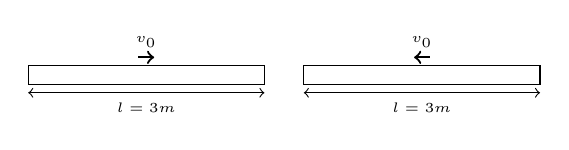
\begin{tikzpicture}
        \draw (0,0) rectangle (3,0.25);
        \draw[<->] (0,-0.1) -- (3,-0.1) node [midway, below] {\tiny $l=3m$};
        \draw[->,thick] (1.4,0.35) -- (1.6,0.35) node [midway, above] {\tiny $v_0$};
        \draw[<->] (3.5,-0.1) -- (6.5,-0.1) node [midway, below] {\tiny $l=3m$};
        \draw[<-,thick] (4.9,0.35) -- (5.1,0.35) node [midway, above] {\tiny $v_0$};
    
        \draw (3.5,0) rectangle (6.5,0.25);
      \end{tikzpicture}
    \end{column}
    \begin{footnotesize}
      \begin{column}{0.49\textwidth}
        $v_0=2.53 \: m/s $; $E= 2\times 10^{11} \: Pa$; $\rho = 7800 \: kg/m^{3}$
      \end{column}
    \end{footnotesize}
  \end{columns}
  \pause
  \centering
  \begin{tikzpicture}[scale=.9]
\begin{groupplot}[group style={group size=2 by 2,
ylabels at=edge left, yticklabels at=edge left,horizontal sep=4.ex,
vertical sep=2ex,xticklabels at=edge bottom,xlabels at=edge bottom},
ymajorgrids=true,xmajorgrids=true,enlargelimits=0,xmin=0.,xmax=6.,xlabel=x (m),
axis on top,scale only axis,width=0.45\linewidth
]
\nextgroupplot[title={(a) time $t = 1.21\times 10^{-4} $ s.},ylabel=$\sigma (Pa)$,]
\addplot[Red,dashed,mark=none,very thick,mark size=3pt] coordinates{(0.0,-1.71821567874e-08) (0.122448979592,4.29553919686e-08) (0.244897959184,1.71821567874e-08) (0.367346938776,8.59107839372e-09) (0.489795918367,-1.71821567874e-08) (0.612244897959,-3.43643135749e-08) (0.734693877551,-2.57732351812e-08) (0.857142857143,0.0) (0.979591836735,0.0) (1.10204081633,-1.71821567874e-08) (1.22448979592,1.71821567874e-08) (1.34693877551,0.0) (1.4693877551,0.0) (1.59183673469,0.0) (1.71428571429,0.0) (1.83673469388,-10490.4174805) (1.95918367347,-180244.445801) (2.08163265306,-1426887.51221) (2.20408163265,-6905937.19482) (2.32653061224,-22447967.5293) (2.44897959184,-53339385.9863) (2.57142857143,-87870025.6348) (2.69387755102,-120363616.943) (2.81632653061,-112137222.29) (2.9387755102,-95318222.0459) (3.0612244898,-95318222.0459) (3.18367346939,-112137222.29) (3.30612244898,-120363616.943) (3.42857142857,-87870025.6348) (3.55102040816,-53339385.9863) (3.67346938776,-22447967.5293) (3.79591836735,-6905937.19482) (3.91836734694,-1426887.51221) (4.04081632653,-180244.445801) (4.16326530612,-10490.4174805) (4.28571428571,0.0) (4.40816326531,0.0) (4.5306122449,0.0) (4.65306122449,0.0) (4.77551020408,1.71821567874e-08) (4.89795918367,-1.71821567874e-08) (5.02040816327,0.0) (5.14285714286,0.0) (5.26530612245,0.0) (5.38775510204,0.0) (5.51020408163,0.0) (5.63265306122,0.0) (5.75510204082,0.0) (5.87755102041,0.0) (6.0,0.0) };
\addplot[Orange,densely dotted,mark=none,very thick,mark size=3pt] coordinates{(0.0,0.0) (0.0606060606061,0.0) (0.121212121212,0.0) (0.181818181818,0.0) (0.242424242424,0.0) (0.30303030303,0.0) (0.363636363636,0.0) (0.424242424242,0.0) (0.484848484848,0.0) (0.545454545455,0.0) (0.606060606061,-8.50429982409e-09) (0.666666666667,-8.50429982409e-09) (0.727272727273,0.0) (0.787878787879,0.0) (0.848484848485,0.0) (0.909090909091,0.0) (0.969696969697,8.50429982409e-09) (1.0303030303,8.50429982409e-09) (1.09090909091,0.0) (1.15151515152,0.0) (1.21212121212,0.0) (1.27272727273,0.0) (1.33333333333,0.0) (1.39393939394,0.0) (1.45454545455,0.0) (1.51515151515,0.0) (1.57575757576,0.0) (1.63636363636,0.0) (1.69696969697,0.0) (1.75757575758,0.0) (1.81818181818,-5499.27353859) (1.87878787879,-5499.27353859) (1.93939393939,-115492.194891) (2.0,-115492.194891) (2.06060606061,-1086898.89312) (2.12121212121,-1086898.89312) (2.18181818182,-6038592.01074) (2.24242424242,-6038592.01074) (2.30303030303,-21882501.2445) (2.36363636364,-21882501.2445) (2.42424242424,-54484376.3113) (2.48484848485,-54484376.3113) (2.54545454545,-94001361.7277) (2.60606060606,-94001361.7277) (2.66666666667,-117371180.654) (2.72727272727,-117371180.654) (2.78787878788,-111648218.334) (2.84848484848,-111648218.334) (2.90909090909,-93365879.3569) (2.9696969697,-93365879.3569) (3.0303030303,-93365879.3569) (3.09090909091,-93365879.3569) (3.15151515152,-111648218.334) (3.21212121212,-111648218.334) (3.27272727273,-117371180.654) (3.33333333333,-117371180.654) (3.39393939394,-94001361.7277) (3.45454545455,-94001361.7277) (3.51515151515,-54484376.3113) (3.57575757576,-54484376.3113) (3.63636363636,-21882501.2445) (3.69696969697,-21882501.2445) (3.75757575758,-6038592.01074) (3.81818181818,-6038592.01074) (3.87878787879,-1086898.89312) (3.93939393939,-1086898.89312) (4.0,-115492.194891) (4.06060606061,-115492.194891) (4.12121212121,-5499.2735386) (4.18181818182,-5499.2735386) (4.24242424242,-8.50429982409e-09) (4.30303030303,-8.50429982409e-09) (4.36363636364,1.70085996482e-08) (4.42424242424,1.70085996482e-08) (4.48484848485,-8.50429982409e-09) (4.54545454545,-8.50429982409e-09) (4.60606060606,0.0) (4.66666666667,0.0) (4.72727272727,0.0) (4.78787878788,0.0) (4.84848484848,0.0) (4.90909090909,0.0) (4.9696969697,0.0) (5.0303030303,0.0) (5.09090909091,0.0) (5.15151515152,0.0) (5.21212121212,0.0) (5.27272727273,0.0) (5.33333333333,0.0) (5.39393939394,0.0) (5.45454545455,0.0) (5.51515151515,0.0) (5.57575757576,0.0) (5.63636363636,0.0) (5.69696969697,0.0) (5.75757575758,0.0) (5.81818181818,0.0) (5.87878787879,0.0) (5.93939393939,0.0) (6.0,0.0) };
\addplot[Duck,solid,mark=*,thick,mark size=2pt] coordinates{(0.0,0.0) (0.0606060606061,0.0) (0.121212121212,0.0) (0.181818181818,0.0) (0.242424242424,0.0) (0.30303030303,0.0) (0.363636363636,-2.55128994723e-08) (0.424242424242,-2.55128994723e-08) (0.484848484848,-2.55128994723e-08) (0.545454545455,-2.55128994723e-08) (0.606060606061,-8.50429982409e-09) (0.666666666667,-8.50429982409e-09) (0.727272727273,-1.70085996482e-08) (0.787878787879,-1.70085996482e-08) (0.848484848485,1.70085996482e-08) (0.909090909091,1.70085996482e-08) (0.969696969697,1.70085996482e-08) (1.0303030303,1.70085996482e-08) (1.09090909091,8.50429982409e-09) (1.15151515152,8.50429982409e-09) (1.21212121212,2.55128994723e-08) (1.27272727273,2.55128994723e-08) (1.33333333333,8.50429982409e-09) (1.39393939394,8.50429982409e-09) (1.45454545455,0.0) (1.51515151515,0.0) (1.57575757576,-2.55128994723e-08) (1.63636363636,-2.55128994723e-08) (1.69696969697,-3.40171992963e-08) (1.75757575758,-3.40171992963e-08) (1.81818181818,-29361.1134112) (1.87878787879,-29361.1134112) (1.93939393939,-478765.91052) (2.0,-478765.91052) (2.06060606061,-3385772.94096) (2.12121212121,-3385772.94096) (2.18181818182,-13710104.1379) (2.24242424242,-13710104.1379) (2.30303030303,-35621767.9306) (2.36363636364,-35621767.9306) (2.42424242424,-64051116.4238) (2.48484848485,-64051116.4238) (2.54545454545,-86391746.7796) (2.60606060606,-86391746.7796) (2.66666666667,-96780453.3284) (2.72727272727,-96780453.3284) (2.78787878788,-99574824.0166) (2.84848484848,-99574824.0166) (2.90909090909,-99976087.4183) (2.9696969697,-99976087.4183) (3.0303030303,-99976087.4183) (3.09090909091,-99976087.4183) (3.15151515152,-99574824.0166) (3.21212121212,-99574824.0166) (3.27272727273,-96780453.3284) (3.33333333333,-96780453.3284) (3.39393939394,-86391746.7796) (3.45454545455,-86391746.7796) (3.51515151515,-64051116.4238) (3.57575757576,-64051116.4238) (3.63636363636,-35621767.9306) (3.69696969697,-35621767.9306) (3.75757575758,-13710104.1379) (3.81818181818,-13710104.1379) (3.87878787879,-3385772.94096) (3.93939393939,-3385772.94096) (4.0,-478765.91052) (4.06060606061,-478765.91052) (4.12121212121,-29361.1134111) (4.18181818182,-29361.1134111) (4.24242424242,0.0) (4.30303030303,0.0) (4.36363636364,3.40171992963e-08) (4.42424242424,3.40171992963e-08) (4.48484848485,-8.50429982409e-09) (4.54545454545,-8.50429982409e-09) (4.60606060606,0.0) (4.66666666667,0.0) (4.72727272727,0.0) (4.78787878788,0.0) (4.84848484848,0.0) (4.90909090909,0.0) (4.9696969697,0.0) (5.0303030303,0.0) (5.09090909091,0.0) (5.15151515152,0.0) (5.21212121212,0.0) (5.27272727273,0.0) (5.33333333333,0.0) (5.39393939394,0.0) (5.45454545455,0.0) (5.51515151515,0.0) (5.57575757576,0.0) (5.63636363636,0.0) (5.69696969697,0.0) (5.75757575758,0.0) (5.81818181818,0.0) (5.87878787879,0.0) (5.93939393939,0.0) (6.0,0.0) };
\addplot[Blue,solid,mark=none,very thick,mark size=3pt] coordinates{(0.0,2.20527643776e-23) (0.122448979592,-4.82139102982e-08) (0.244897959184,-3.61604327236e-08) (0.367346938776,2.41069551491e-08) (0.489795918367,-3.61604327236e-08) (0.612244897959,-2.41069551491e-08) (0.734693877551,1.20534775745e-08) (0.857142857143,-1.20534775745e-08) (0.979591836735,1.20534775745e-08) (1.10204081633,1.20534775745e-08) (1.22448979592,2.41069551491e-08) (1.34693877551,2.41069551491e-08) (1.4693877551,-6.30078982218e-24) (1.59183673469,-6.30078982218e-24) (1.71428571429,1.20534775745e-08) (1.83673469388,-2.41069551491e-08) (1.95918367347,0.0) (2.08163265306,0.0) (2.20408163265,1.57519745555e-23) (2.32653061224,1.57519745555e-23) (2.44897959184,-100000000.0) (2.57142857143,-100000000.0) (2.69387755102,-100000000.0) (2.81632653061,-100000000.0) (2.9387755102,-100000000.0) (3.0612244898,-100000000.0) (3.18367346939,-100000000.0) (3.30612244898,-100000000.0) (3.42857142857,-100000000.0) (3.55102040816,-100000000.0) (3.67346938776,-1.26015796444e-23) (3.79591836735,1.20534775745e-08) (3.91836734694,1.20534775745e-08) (4.04081632653,-3.61604327236e-08) (4.16326530612,1.41767770999e-23) (4.28571428571,-1.41767770999e-23) (4.40816326531,-2.41069551491e-08) (4.5306122449,-1.20534775745e-08) (4.65306122449,1.20534775745e-08) (4.77551020408,-1.89023694665e-23) (4.89795918367,-1.20534775745e-08) (5.02040816327,-2.41069551491e-08) (5.14285714286,3.61604327236e-08) (5.26530612245,-1.20534775745e-08) (5.38775510204,-1.89023694665e-23) (5.51020408163,2.41069551491e-08) (5.63265306122,-1.89023694665e-23) (5.75510204082,-1.20534775745e-08) (5.87755102041,2.41069551491e-08) (6.0,-1.57519745555e-23) };
\addplot[Purple,solid,mark=|,very thick,mark size=3pt] coordinates{(0.0,1.19548956657e-11) (0.0606060606061,-1.19548956657e-11) (0.121212121212,-9.04006220054e-09) (0.181818181818,-1.50668929485e-08) (0.242424242424,-2.01489535813e-08) (0.30303030303,-4.01184342914e-08) (0.363636363636,-3.98015720808e-08) (0.424242424242,-4.4572770941e-08) (0.484848484848,-3.05172621658e-08) (0.545454545455,-2.9750125707e-08) (0.606060606061,-1.89546709994e-08) (0.666666666667,-5.1522841497e-09) (0.727272727273,-1.17903779092e-08) (0.787878787879,-1.23165772399e-08) (0.848484848485,-2.54735836451e-08) (0.909090909091,1.36662849606e-09) (0.969696969697,3.64534656085e-08) (1.0303030303,2.38139222642e-08) (1.09090909091,2.4282772581e-08) (1.15151515152,2.39311377172e-08) (1.21212121212,1.22434109794e-08) (1.27272727273,1.18635441697e-08) (1.33333333333,1.25831714133e-08) (1.39393939394,1.15237837358e-08) (1.45454545455,2.73711934302e-08) (1.51515151515,2.08427168679e-08) (1.57575757576,9.62496696607e-09) (1.63636363636,1.4481988183e-08) (1.69696969697,2.10480996765e-08) (1.75757575758,1.51123330472e-08) (1.81818181818,-3666.24444723) (1.87878787879,-10998.7333417) (1.93939393939,-100618.042052) (2.0,-262747.518718) (2.06060606061,-1140066.23626) (2.12121212121,-2551162.98795) (2.18181818182,-6952185.18376) (2.24242424242,-13110550.493) (2.30303030303,-25132333.1147) (2.36363636364,-39370855.3165) (2.42424242424,-56894854.8287) (2.48484848485,-73865127.936) (2.54545454545,-86159824.58) (2.60606060606,-95498106.6287) (2.66666666667,-98513982.445) (2.72727272727,-100261419.266) (2.78787878788,-100094961.189) (2.84848484848,-100070640.631) (2.90909090909,-100007508.136) (2.9696969697,-99998390.4883) (3.0303030303,-99998390.4883) (3.09090909091,-100007508.136) (3.15151515152,-100070640.631) (3.21212121212,-100094961.189) (3.27272727273,-100261419.266) (3.33333333333,-98513982.445) (3.39393939394,-95498106.6287) (3.45454545455,-86159824.58) (3.51515151515,-73865127.936) (3.57575757576,-56894854.8287) (3.63636363636,-39370855.3165) (3.69696969697,-25132333.1147) (3.75757575758,-13110550.493) (3.81818181818,-6952185.18376) (3.87878787879,-2551162.98795) (3.93939393939,-1140066.23626) (4.0,-262747.518718) (4.06060606061,-100618.042052) (4.12121212121,-10998.7333417) (4.18181818182,-3666.24444723) (4.24242424242,6.0265548658e-09) (4.30303030303,6.02692270874e-09) (4.36363636364,2.0086063933e-09) (4.42424242424,-1.40620839678e-08) (4.48484848485,0.0) (4.54545454545,0.0) (4.60606060606,0.0) (4.66666666667,0.0) (4.72727272727,0.0) (4.78787878788,0.0) (4.84848484848,0.0) (4.90909090909,0.0) (4.9696969697,0.0) (5.0303030303,0.0) (5.09090909091,0.0) (5.15151515152,0.0) (5.21212121212,0.0) (5.27272727273,0.0) (5.33333333333,0.0) (5.39393939394,0.0) (5.45454545455,0.0) (5.51515151515,0.0) (5.57575757576,0.0) (5.63636363636,0.0) (5.69696969697,0.0) (5.75757575758,0.0) (5.81818181818,0.0) (5.87878787879,0.0) (5.93939393939,-6.02672729218e-09) (6.0,-6.02675028236e-09) };
\addplot[Green,only marks,mark=x,thick,mark size=3pt] coordinates{(0.0,-2.10935857555e-08) (0.0606060606061,-3.01336939364e-09) (0.121212121212,-2.50486330846e-08) (0.181818181818,-2.31652772136e-08) (0.242424242424,-1.40780851359e-08) (0.30303030303,-1.00288700132e-08) (0.363636363636,-4.37173981561e-08) (0.424242424242,-2.86034672912e-08) (0.484848484848,7.15675230988e-09) (0.545454545455,1.69502028392e-08) (0.606060606061,-4.36938562077e-08) (0.666666666667,-5.27339643886e-08) (0.727272727273,3.35237345042e-08) (0.787878787879,3.87971309431e-08) (0.848484848485,-1.48785113811e-08) (0.909090909091,-9.22844376801e-09) (0.969696969697,5.57002498855e-08) (1.0303030303,8.8941481009e-08) (1.09090909091,-5.9255084092e-08) (1.15151515152,-3.71727365043e-08) (1.21212121212,2.8956596517e-09) (1.27272727273,2.12112954974e-08) (1.33333333333,3.92679699108e-08) (1.39393939394,8.94594038736e-09) (1.45454545455,-2.01048239232e-08) (1.51515151515,-2.8109086375e-08) (1.57575757576,5.15568669692e-09) (1.63636363636,-5.15568669692e-09) (1.69696969697,1.90925201425e-08) (1.75757575758,5.0144350066e-09) (1.81818181818,-1.05467928777e-08) (1.87878787879,-1.35601622714e-08) (1.93939393939,-4.89672526466e-09) (2.0,-1.92102298844e-08) (2.06060606061,6.19153242599e-09) (2.12121212121,-6.19153242599e-09) (2.18181818182,-1.77741710328e-08) (2.24242424242,-3.04397392654e-08) (2.30303030303,1.76093773941e-08) (2.36363636364,6.49757775503e-09) (2.42424242424,-100000000.0) (2.48484848485,-100000000.0) (2.54545454545,-100000000.0) (2.60606060606,-100000000.0) (2.66666666667,-100000000.0) (2.72727272727,-100000000.0) (2.78787878788,-100000000.0) (2.84848484848,-100000000.0) (2.90909090909,-100000000.0) (2.9696969697,-100000000.0) (3.0303030303,-100000000.0) (3.09090909091,-100000000.0) (3.15151515152,-100000000.0) (3.21212121212,-100000000.0) (3.27272727273,-100000000.0) (3.33333333333,-100000000.0) (3.39393939394,-100000000.0) (3.45454545455,-100000000.0) (3.51515151515,-100000000.0) (3.57575757576,-100000000.0) (3.63636363636,0.0) (3.69696969697,0.0) (3.75757575758,0.0) (3.81818181818,0.0) (3.87878787879,0.0) (3.93939393939,0.0) (4.0,-6.02673878727e-09) (4.06060606061,-1.80802163618e-08) (4.12121212121,1.80802163618e-08) (4.18181818182,6.02673878727e-09) (4.24242424242,-1.64793638714e-10) (4.30303030303,-2.39421615104e-08) (4.36363636364,2.21058895361e-08) (4.42424242424,2.6108020762e-08) (4.48484848485,-1.10176318455e-08) (4.54545454545,-1.30893233036e-08) (4.60606060606,2.41069551491e-08) (4.66666666667,2.41069551491e-08) (4.72727272727,-2.41069551491e-08) (4.78787878788,-2.41069551491e-08) (4.84848484848,0.0) (4.90909090909,0.0) (4.9696969697,0.0) (5.0303030303,0.0) (5.09090909091,0.0) (5.15151515152,0.0) (5.21212121212,0.0) (5.27272727273,0.0) (5.33333333333,0.0) (5.39393939394,0.0) (5.45454545455,0.0) (5.51515151515,0.0) (5.57575757576,0.0) (5.63636363636,0.0) (5.69696969697,0.0) (5.75757575758,0.0) (5.81818181818,0.0) (5.87878787879,0.0) (5.93939393939,0.0) (6.0,0.0) };
\addplot[black,solid,mark=pentagone*,thin,mark size=3pt] coordinates{(0.0,-0.0) (0.122448979592,-0.0) (0.244897959184,-0.0) (0.367346938776,-0.0) (0.489795918367,-0.0) (0.612244897959,-0.0) (0.734693877551,-0.0) (0.857142857143,-0.0) (0.979591836735,-0.0) (1.10204081633,-0.0) (1.22448979592,-0.0) (1.34693877551,-0.0) (1.4693877551,-0.0) (1.59183673469,-0.0) (1.71428571429,-0.0) (1.83673469388,-0.0) (1.95918367347,-0.0) (2.08163265306,-0.0) (2.20408163265,-0.0) (2.32653061224,-0.0) (2.44897959184,-100000000.0) (2.57142857143,-100000000.0) (2.69387755102,-100000000.0) (2.81632653061,-100000000.0) (2.9387755102,-100000000.0) (3.0612244898,-100000000.0) (3.18367346939,-100000000.0) (3.30612244898,-100000000.0) (3.42857142857,-100000000.0) (3.55102040816,-100000000.0) (3.67346938776,-0.0) (3.79591836735,-0.0) (3.91836734694,-0.0) (4.04081632653,-0.0) (4.16326530612,-0.0) (4.28571428571,-0.0) (4.40816326531,-0.0) (4.5306122449,-0.0) (4.65306122449,-0.0) (4.77551020408,-0.0) (4.89795918367,-0.0) (5.02040816327,-0.0) (5.14285714286,-0.0) (5.26530612245,-0.0) (5.38775510204,-0.0) (5.51020408163,-0.0) (5.63265306122,-0.0) (5.75510204082,-0.0) (5.87755102041,-0.0) (6.0,-0.0) };
\nextgroupplot[title={(b) time $t = 4.84\times 10^{-4} $ s.},]
\addplot[Red,dashed,mark=none,very thick,mark size=3pt] coordinates{(0.0,-8.59107839372e-09) (0.122448979592,4.29553919686e-08) (0.244897959184,2.57732351812e-08) (0.367346938776,8.59107839372e-09) (0.489795918367,-8.59107839372e-09) (0.612244897959,-1.23054636115) (0.734693877551,-40.5516402702) (0.857142857143,-640.213875183) (0.979591836735,-6438.55873936) (1.10204081633,-46257.8011138) (1.22448979592,-252333.895514) (1.34693877551,-1084103.88038) (1.4693877551,-3755013.24106) (1.59183673469,-10642636.9901) (1.71428571429,-24916947.9583) (1.83673469388,-48387367.3518) (1.95918367347,-78275857.836) (2.08163265306,-105019368.728) (2.20408163265,-119223316.597) (2.32653061224,-113889153.316) (2.44897959184,-103439986.404) (2.57142857143,-92963963.4978) (2.69387755102,-96202736.2231) (2.81632653061,-98859035.7487) (2.9387755102,-103034799.977) (3.0612244898,-103034799.977) (3.18367346939,-98859035.7487) (3.30612244898,-96202736.2231) (3.42857142857,-92963963.4978) (3.55102040816,-103439986.404) (3.67346938776,-113889153.316) (3.79591836735,-119223316.597) (3.91836734694,-105019368.728) (4.04081632653,-78275857.836) (4.16326530612,-48387367.3518) (4.28571428571,-24916947.9583) (4.40816326531,-10642636.9901) (4.5306122449,-3755013.24106) (4.65306122449,-1084103.88038) (4.77551020408,-252333.895514) (4.89795918367,-46257.8011138) (5.02040816327,-6438.55873932) (5.14285714286,-640.213875175) (5.26530612245,-40.5516402702) (5.38775510204,-1.23054632679) (5.51020408163,0.0) (5.63265306122,0.0) (5.75510204082,0.0) (5.87755102041,0.0) (6.0,0.0) };
\addplot[Orange,densely dotted,mark=none,very thick,mark size=3pt] coordinates{(0.0,0.0) (0.0606060606061,0.0) (0.121212121212,0.0) (0.181818181818,0.0) (0.242424242424,0.0) (0.30303030303,0.0) (0.363636363636,0.0) (0.424242424242,0.0) (0.484848484848,0.0) (0.545454545455,0.0) (0.606060606061,-0.302430335559) (0.666666666667,-0.302430335559) (0.727272727273,-12.3996438685) (0.787878787879,-12.3996438685) (0.848484848485,-240.230497765) (0.909090909091,-240.230497765) (0.969696969697,-2921.77951372) (1.0303030303,-2921.77951372) (1.09090909091,-24993.4810877) (1.15151515152,-24993.4810877) (1.21212121212,-159637.896304) (1.27272727273,-159637.896304) (1.33333333333,-788716.389772) (1.39393939394,-788716.389772) (1.45454545455,-3080624.98423) (1.51515151515,-3080624.98423) (1.57575757576,-9638116.18636) (1.63636363636,-9638116.18636) (1.69696969697,-24323655.3377) (1.75757575758,-24323655.3377) (1.81818181818,-49636559.9635) (1.87878787879,-49636559.9635) (1.93939393939,-81867011.1376) (2.0,-81867011.1376) (2.06060606061,-109111634.24) (2.12121212121,-109111634.24) (2.18181818182,-118687950.99) (2.24242424242,-118687950.99) (2.30303030303,-110105828.793) (2.36363636364,-110105828.793) (2.42424242424,-97435608.9991) (2.48484848485,-97435608.9991) (2.54545454545,-94244104.916) (2.60606060606,-94244104.916) (2.66666666667,-99081654.2889) (2.72727272727,-99081654.2889) (2.78787878788,-101740412.886) (2.84848484848,-101740412.886) (2.90909090909,-100070314.798) (2.9696969697,-100070314.798) (3.0303030303,-100070314.798) (3.09090909091,-100070314.798) (3.15151515152,-101740412.886) (3.21212121212,-101740412.886) (3.27272727273,-99081654.2889) (3.33333333333,-99081654.2889) (3.39393939394,-94244104.916) (3.45454545455,-94244104.916) (3.51515151515,-97435608.9991) (3.57575757576,-97435608.9991) (3.63636363636,-110105828.793) (3.69696969697,-110105828.793) (3.75757575758,-118687950.99) (3.81818181818,-118687950.99) (3.87878787879,-109111634.24) (3.93939393939,-109111634.24) (4.0,-81867011.1376) (4.06060606061,-81867011.1376) (4.12121212121,-49636559.9635) (4.18181818182,-49636559.9635) (4.24242424242,-24323655.3377) (4.30303030303,-24323655.3377) (4.36363636364,-9638116.18636) (4.42424242424,-9638116.18636) (4.48484848485,-3080624.98423) (4.54545454545,-3080624.98423) (4.60606060606,-788716.389772) (4.66666666667,-788716.389772) (4.72727272727,-159637.896304) (4.78787878788,-159637.896304) (4.84848484848,-24993.4810877) (4.90909090909,-24993.4810877) (4.9696969697,-2921.7795137) (5.0303030303,-2921.7795137) (5.09090909091,-240.230497756) (5.15151515152,-240.230497756) (5.21212121212,-12.3996438685) (5.27272727273,-12.3996438685) (5.33333333333,-0.302430344063) (5.39393939394,-0.302430344063) (5.45454545455,0.0) (5.51515151515,0.0) (5.57575757576,0.0) (5.63636363636,0.0) (5.69696969697,0.0) (5.75757575758,0.0) (5.81818181818,0.0) (5.87878787879,0.0) (5.93939393939,0.0) (6.0,0.0) };
\addplot[Duck,solid,mark=*,thick,mark size=2pt] coordinates{(0.0,-8.50429982409e-09) (0.0606060606061,-8.50429982409e-09) (0.121212121212,-2.55128994723e-08) (0.181818181818,-2.55128994723e-08) (0.242424242424,-1.70085996482e-08) (0.30303030303,-1.70085996482e-08) (0.363636363636,-5.10257989445e-08) (0.424242424242,-5.10257989445e-08) (0.484848484848,-3.40171992963e-08) (0.545454545455,-3.40171992963e-08) (0.606060606061,-7.54315610416) (0.666666666667,-7.54315610416) (0.727272727273,-243.074356172) (0.787878787879,-243.074356172) (0.848484848485,-3634.66708743) (0.909090909091,-3634.66708743) (0.969696969697,-33492.7067527) (1.0303030303,-33492.7067527) (1.09090909091,-213117.914955) (1.15151515152,-213117.914955) (1.21212121212,-995090.547212) (1.27272727273,-995090.547212) (1.33333333333,-3540220.94427) (1.39393939394,-3540220.94427) (1.45454545455,-9852354.5249) (1.51515151515,-9852354.5249) (1.57575757576,-21906072.5461) (1.63636363636,-21906072.5461) (1.69696969697,-39711055.8831) (1.75757575758,-39711055.8831) (1.81818181818,-60065449.8718) (1.87878787879,-60065449.8718) (1.93939393939,-78032993.3013) (2.0,-78032993.3013) (2.06060606061,-90231435.0995) (2.12121212121,-90231435.0995) (2.18181818182,-96567889.7944) (2.24242424242,-96567889.7944) (2.30303030303,-99068409.7758) (2.36363636364,-99068409.7758) (2.42424242424,-99809735.7536) (2.48484848485,-99809735.7536) (2.54545454545,-99971826.9969) (2.60606060606,-99971826.9969) (2.66666666667,-99997149.6439) (2.72727272727,-99997149.6439) (2.78787878788,-99999824.5348) (2.84848484848,-99999824.5348) (2.90909090909,-99999994.876) (2.9696969697,-99999994.876) (3.0303030303,-99999994.876) (3.09090909091,-99999994.876) (3.15151515152,-99999824.5348) (3.21212121212,-99999824.5348) (3.27272727273,-99997149.6439) (3.33333333333,-99997149.6439) (3.39393939394,-99971826.9969) (3.45454545455,-99971826.9969) (3.51515151515,-99809735.7536) (3.57575757576,-99809735.7536) (3.63636363636,-99068409.7758) (3.69696969697,-99068409.7758) (3.75757575758,-96567889.7944) (3.81818181818,-96567889.7944) (3.87878787879,-90231435.0995) (3.93939393939,-90231435.0995) (4.0,-78032993.3013) (4.06060606061,-78032993.3013) (4.12121212121,-60065449.8718) (4.18181818182,-60065449.8718) (4.24242424242,-39711055.8831) (4.30303030303,-39711055.8831) (4.36363636364,-21906072.5461) (4.42424242424,-21906072.5461) (4.48484848485,-9852354.5249) (4.54545454545,-9852354.5249) (4.60606060606,-3540220.94427) (4.66666666667,-3540220.94427) (4.72727272727,-995090.547212) (4.78787878788,-995090.547212) (4.84848484848,-213117.914955) (4.90909090909,-213117.914955) (4.9696969697,-33492.7067527) (5.0303030303,-33492.7067527) (5.09090909091,-3634.66708747) (5.15151515152,-3634.66708747) (5.21212121212,-243.074356181) (5.27272727273,-243.074356181) (5.33333333333,-7.54315609566) (5.39393939394,-7.54315609566) (5.45454545455,0.0) (5.51515151515,0.0) (5.57575757576,0.0) (5.63636363636,0.0) (5.69696969697,0.0) (5.75757575758,0.0) (5.81818181818,0.0) (5.87878787879,0.0) (5.93939393939,0.0) (6.0,0.0) };
\addplot[Blue,solid,mark=none,very thick,mark size=3pt] coordinates{(0.0,1.89023694665e-23) (0.122448979592,6.30078982218e-23) (0.244897959184,-2.20527643776e-23) (0.367346938776,1.08481298171e-07) (0.489795918367,-6.02673878727e-08) (0.612244897959,-3.78047389331e-23) (0.734693877551,-2.41069551491e-08) (0.857142857143,-1.20534775745e-08) (0.979591836735,3.61604327236e-08) (1.10204081633,-1.20534775745e-08) (1.22448979592,3.61604327236e-08) (1.34693877551,-3.15039491109e-24) (1.4693877551,1.20534775745e-08) (1.59183673469,-6.30078982218e-24) (1.71428571429,2.41069551491e-08) (1.83673469388,-100000000.0) (1.95918367347,-100000000.0) (2.08163265306,-100000000.0) (2.20408163265,-100000000.0) (2.32653061224,-100000000.0) (2.44897959184,-100000000.0) (2.57142857143,-100000000.0) (2.69387755102,-100000000.0) (2.81632653061,-100000000.0) (2.9387755102,-100000000.0) (3.0612244898,-100000000.0) (3.18367346939,-100000000.0) (3.30612244898,-100000000.0) (3.42857142857,-100000000.0) (3.55102040816,-100000000.0) (3.67346938776,-100000000.0) (3.79591836735,-100000000.0) (3.91836734694,-100000000.0) (4.04081632653,-100000000.0) (4.16326530612,-100000000.0) (4.28571428571,1.20534775745e-08) (4.40816326531,-3.61604327236e-08) (4.5306122449,-6.30078982218e-24) (4.65306122449,-2.41069551491e-08) (4.77551020408,-1.20534775745e-08) (4.89795918367,-4.82139102982e-08) (5.02040816327,-3.30791465665e-23) (5.14285714286,2.41069551491e-08) (5.26530612245,-4.82139102982e-08) (5.38775510204,2.41069551491e-08) (5.51020408163,-3.15039491109e-23) (5.63265306122,-3.61604327236e-08) (5.75510204082,2.41069551491e-08) (5.87755102041,3.61604327236e-08) (6.0,-1.20534775745e-08) };
\addplot[Purple,solid,mark=|,very thick,mark size=3pt] coordinates{(0.0,-6.62623071053e-10) (0.0606060606061,-1.13908545035e-08) (0.121212121212,-1.03251991157e-08) (0.181818181818,-2.58352336079e-08) (0.242424242424,-5.14381821174e-08) (0.30303030303,-4.4989638479e-08) (0.363636363636,-5.34390135805e-08) (0.424242424242,-5.50422845904e-08) (0.484848484848,-2.21025908105e-08) (0.545454545455,-3.81647970622e-08) (0.606060606061,-0.201620272159) (0.666666666667,-0.604860699987) (0.727272727273,-10.6858719382) (0.787878787879,-29.9070000639) (0.848484848485,-256.986134699) (0.909090909091,-668.206763393) (0.969696969697,-3715.07114041) (1.0303030303,-8933.82287809) (1.09090909091,-36066.6707163) (1.15151515152,-79819.6254771) (1.21212121212,-248965.8763) (1.27272727273,-504422.520742) (1.33333333333,-1263261.9825) (1.39393939394,-2330406.84983) (1.45454545455,-4810891.93605) (1.51515151515,-8037941.25365) (1.57575757576,-13953612.4785) (1.63636363636,-21022005.3552) (1.69696969697,-31228050.0112) (1.75757575758,-42338748.4528) (1.81818181818,-54831068.3252) (1.87878787879,-67114743.6608) (1.93939393939,-77590809.6787) (2.0,-86813439.423) (2.06060606061,-92463242.0658) (2.12121212121,-96885420.8686) (2.18181818182,-98592164.6111) (2.24242424242,-99785509.2556) (2.30303030303,-99950031.6158) (2.36363636364,-100067351.927) (2.42424242424,-100025492.446) (2.48484848485,-100011084.154) (2.54545454545,-100002494.767) (2.60606060606,-99999559.9552) (2.66666666667,-99999874.1387) (2.72727272727,-99999912.159) (2.78787878788,-99999990.2886) (2.84848484848,-100000001.919) (2.90909090909,-100000000.164) (2.9696969697,-100000000.078) (3.0303030303,-100000000.078) (3.09090909091,-100000000.164) (3.15151515152,-100000001.919) (3.21212121212,-99999990.2886) (3.27272727273,-99999912.159) (3.33333333333,-99999874.1387) (3.39393939394,-99999559.9552) (3.45454545455,-100002494.767) (3.51515151515,-100011084.154) (3.57575757576,-100025492.446) (3.63636363636,-100067351.927) (3.69696969697,-99950031.6158) (3.75757575758,-99785509.2556) (3.81818181818,-98592164.6111) (3.87878787879,-96885420.8686) (3.93939393939,-92463242.0658) (4.0,-86813439.423) (4.06060606061,-77590809.6787) (4.12121212121,-67114743.6608) (4.18181818182,-54831068.3252) (4.24242424242,-42338748.4528) (4.30303030303,-31228050.0112) (4.36363636364,-21022005.3552) (4.42424242424,-13953612.4785) (4.48484848485,-8037941.25365) (4.54545454545,-4810891.93605) (4.60606060606,-2330406.84983) (4.66666666667,-1263261.9825) (4.72727272727,-504422.520742) (4.78787878788,-248965.8763) (4.84848484848,-79819.6254771) (4.90909090909,-36066.6707163) (4.9696969697,-8933.82287811) (5.0303030303,-3715.07114043) (5.09090909091,-668.206763402) (5.15151515152,-256.986134702) (5.21212121212,-29.9070000726) (5.27272727273,-10.6858719415) (5.33333333333,-0.604860674869) (5.39393939394,-0.201620224956) (5.45454545455,0.0) (5.51515151515,0.0) (5.57575757576,0.0) (5.63636363636,0.0) (5.69696969697,0.0) (5.75757575758,0.0) (5.81818181818,0.0) (5.87878787879,0.0) (5.93939393939,-6.02673878726e-09) (6.0,-6.02673878728e-09) };
\addplot[Green,only marks,mark=x,thick,mark size=3pt] coordinates{(0.0,-4.24785031222e-08) (0.0606060606061,-5.39493174741e-08) (0.121212121212,4.17860387809e-08) (0.181818181818,3.05348266663e-08) (0.242424242424,-1.08312734142e-08) (0.30303030303,1.08312734142e-08) (0.363636363636,-1.37558777075e-08) (0.424242424242,-1.03510774416e-08) (0.484848484848,-6.55691082182e-08) (0.545454545455,-5.49656675272e-08) (0.606060606061,-4.3242145073e-08) (0.666666666667,-2.90787203742e-08) (0.727272727273,-3.72459372501e-08) (0.787878787879,-3.50749281972e-08) (0.848484848485,-3.29863159637e-09) (0.909090909091,-2.08083235527e-08) (0.969696969697,1.35203892531e-08) (1.0303030303,1.0586565896e-08) (1.09090909091,1.42527645537e-09) (1.15151515152,-1.42527645537e-09) (1.21212121212,-4.952752343e-09) (1.27272727273,4.952752343e-09) (1.33333333333,4.19430157571e-08) (1.39393939394,3.03778496901e-08) (1.45454545455,3.00669764225e-08) (1.51515151515,4.22538890248e-08) (1.57575757576,-1.21426105178e-08) (1.63636363636,-1.19643446313e-08) (1.69696969697,1.70747866461e-08) (1.75757575758,3.1139123652e-08) (1.81818181818,-100000000.0) (1.87878787879,-100000000.0) (1.93939393939,-100000000.0) (2.0,-100000000.0) (2.06060606061,-100000000.0) (2.12121212121,-100000000.0) (2.18181818182,-100000000.0) (2.24242424242,-100000000.0) (2.30303030303,-100000000.0) (2.36363636364,-100000000.0) (2.42424242424,-100000000.0) (2.48484848485,-100000000.0) (2.54545454545,-100000000.0) (2.60606060606,-100000000.0) (2.66666666667,-100000000.0) (2.72727272727,-100000000.0) (2.78787878788,-100000000.0) (2.84848484848,-100000000.0) (2.90909090909,-100000000.0) (2.9696969697,-100000000.0) (3.0303030303,-100000000.0) (3.09090909091,-100000000.0) (3.15151515152,-100000000.0) (3.21212121212,-100000000.0) (3.27272727273,-100000000.0) (3.33333333333,-100000000.0) (3.39393939394,-100000000.0) (3.45454545455,-100000000.0) (3.51515151515,-100000000.0) (3.57575757576,-100000000.0) (3.63636363636,-100000000.0) (3.69696969697,-100000000.0) (3.75757575758,-100000000.0) (3.81818181818,-100000000.0) (3.87878787879,-100000000.0) (3.93939393939,-100000000.0) (4.0,-100000000.0) (4.06060606061,-100000000.0) (4.12121212121,-100000000.0) (4.18181818182,-100000000.0) (4.24242424242,-4.81448937659e-09) (4.30303030303,4.81448937659e-09) (4.36363636364,-1.4144710689e-09) (4.42424242424,1.4144710689e-09) (4.48484848485,1.2195740833e-08) (4.54545454545,1.19112143161e-08) (4.60606060606,-3.0110151988e-08) (4.66666666667,-4.22107134593e-08) (4.72727272727,-6.28570021954e-09) (4.78787878788,-1.78212549295e-08) (4.84848484848,8.92239843897e-09) (4.90909090909,1.51845567101e-08) (4.9696969697,-4.2375507098e-09) (5.0303030303,4.2375507098e-09) (5.09090909091,-1.35601622714e-08) (5.15151515152,-1.05467928777e-08) (5.21212121212,1.20534775745e-08) (5.27272727273,3.61604327236e-08) (5.33333333333,-4.21871715109e-08) (5.39393939394,-3.01336939364e-08) (5.45454545455,0.0) (5.51515151515,0.0) (5.57575757576,0.0) (5.63636363636,0.0) (5.69696969697,0.0) (5.75757575758,0.0) (5.81818181818,0.0) (5.87878787879,0.0) (5.93939393939,0.0) (6.0,0.0) };
\addplot[black,solid,mark=pentagone*,thin,mark size=3pt] coordinates{(0.0,-0.0) (0.122448979592,-0.0) (0.244897959184,-0.0) (0.367346938776,-0.0) (0.489795918367,-0.0) (0.612244897959,-0.0) (0.734693877551,-0.0) (0.857142857143,-0.0) (0.979591836735,-0.0) (1.10204081633,-0.0) (1.22448979592,-0.0) (1.34693877551,-0.0) (1.4693877551,-0.0) (1.59183673469,-0.0) (1.71428571429,-0.0) (1.83673469388,-100000000.0) (1.95918367347,-100000000.0) (2.08163265306,-100000000.0) (2.20408163265,-100000000.0) (2.32653061224,-100000000.0) (2.44897959184,-100000000.0) (2.57142857143,-100000000.0) (2.69387755102,-100000000.0) (2.81632653061,-100000000.0) (2.9387755102,-100000000.0) (3.0612244898,-100000000.0) (3.18367346939,-100000000.0) (3.30612244898,-100000000.0) (3.42857142857,-100000000.0) (3.55102040816,-100000000.0) (3.67346938776,-100000000.0) (3.79591836735,-100000000.0) (3.91836734694,-100000000.0) (4.04081632653,-100000000.0) (4.16326530612,-100000000.0) (4.28571428571,-0.0) (4.40816326531,-0.0) (4.5306122449,-0.0) (4.65306122449,-0.0) (4.77551020408,-0.0) (4.89795918367,-0.0) (5.02040816327,-0.0) (5.14285714286,-0.0) (5.26530612245,-0.0) (5.38775510204,-0.0) (5.51020408163,-0.0) (5.63265306122,-0.0) (5.75510204082,-0.0) (5.87755102041,-0.0) (6.0,-0.0) };
\nextgroupplot[ylabel=v (m/s),]
\addplot[Red,dashed,mark=none,very thick,mark size=3pt] coordinates{(0.0,2.53184841771) (0.122448979592,2.53184841771) (0.244897959184,2.53184841771) (0.367346938776,2.53184841771) (0.489795918367,2.53184841771) (0.612244897959,2.53184841771) (0.734693877551,2.53184841771) (0.857142857143,2.53184841771) (0.979591836735,2.53184841771) (1.10204081633,2.53184841771) (1.22448979592,2.53184841771) (1.34693877551,2.53184841771) (1.4693877551,2.53184841771) (1.59183673469,2.53184841771) (1.71428571429,2.53184841771) (1.83673469388,2.53168422771) (1.95918367347,2.52888333949) (2.08163265306,2.50699777845) (2.20408163265,2.40545109318) (2.32653061224,2.08436306275) (2.44897959184,1.45719589947) (2.57142857143,0.368133294256) (2.69387755102,0.0385943080031) (2.81632653061,-0.906077680431) (2.9387755102,0.154976042597) (3.0612244898,-0.154976042597) (3.18367346939,0.906077680431) (3.30612244898,-0.0385943080031) (3.42857142857,-0.368133294256) (3.55102040816,-1.45719589947) (3.67346938776,-2.08436306275) (3.79591836735,-2.40545109318) (3.91836734694,-2.50699777845) (4.04081632653,-2.52888333949) (4.16326530612,-2.53168422771) (4.28571428571,-2.53184841771) (4.40816326531,-2.53184841771) (4.5306122449,-2.53184841771) (4.65306122449,-2.53184841771) (4.77551020408,-2.53184841771) (4.89795918367,-2.53184841771) (5.02040816327,-2.53184841771) (5.14285714286,-2.53184841771) (5.26530612245,-2.53184841771) (5.38775510204,-2.53184841771) (5.51020408163,-2.53184841771) (5.63265306122,-2.53184841771) (5.75510204082,-2.53184841771) (5.87755102041,-2.53184841771) (6.0,-2.53184841771) };
\addplot[Orange,densely dotted,mark=none,very thick,mark size=3pt] coordinates{(0.0,2.53184841771) (0.0606060606061,2.53184841771) (0.121212121212,2.53184841771) (0.181818181818,2.53184841771) (0.242424242424,2.53184841771) (0.30303030303,2.53184841771) (0.363636363636,2.53184841771) (0.424242424242,2.53184841771) (0.484848484848,2.53184841771) (0.545454545455,2.53184841771) (0.606060606061,2.53184841771) (0.666666666667,2.53184841771) (0.727272727273,2.53184841771) (0.787878787879,2.53184841771) (0.848484848485,2.53184841771) (0.909090909091,2.53184841771) (0.969696969697,2.53184841771) (1.0303030303,2.53184841771) (1.09090909091,2.53184841771) (1.15151515152,2.53184841771) (1.21212121212,2.53184841771) (1.27272727273,2.53184841771) (1.33333333333,2.53184841771) (1.39393939394,2.53184841771) (1.45454545455,2.53184841771) (1.51515151515,2.53184841771) (1.57575757576,2.53184841771) (1.63636363636,2.53184841771) (1.69696969697,2.53184841771) (1.75757575758,2.53184841771) (1.81818181818,2.53180200348) (1.87878787879,2.53170917501) (1.93939393939,2.53075014243) (2.0,2.52892490574) (2.06060606061,2.52011291678) (2.12121212121,2.50431417554) (2.18181818182,2.45734572485) (2.24242424242,2.37920756473) (2.30303030303,2.21852587251) (2.36363636364,1.97530064819) (2.42424242424,1.62562122327) (2.48484848485,1.16948759776) (2.54545454545,0.652158035596) (2.60606060606,0.0736325367928) (2.66666666667,-0.209593400584) (2.72727272727,-0.197519776535) (2.78787878788,-0.41340730943) (2.84848484848,-0.857255999272) (2.90909090909,-0.176423153717) (2.9696969697,1.62909122723) (3.0303030303,-1.62909122723) (3.09090909091,0.176423153717) (3.15151515152,0.857255999272) (3.21212121212,0.41340730943) (3.27272727273,0.197519776535) (3.33333333333,0.209593400584) (3.39393939394,-0.0736325367928) (3.45454545455,-0.652158035596) (3.51515151515,-1.16948759776) (3.57575757576,-1.62562122327) (3.63636363636,-1.97530064819) (3.69696969697,-2.21852587251) (3.75757575758,-2.37920756473) (3.81818181818,-2.45734572485) (3.87878787879,-2.50431417554) (3.93939393939,-2.52011291678) (4.0,-2.52892490574) (4.06060606061,-2.53075014243) (4.12121212121,-2.53170917501) (4.18181818182,-2.53180200348) (4.24242424242,-2.53184841771) (4.30303030303,-2.53184841771) (4.36363636364,-2.53184841771) (4.42424242424,-2.53184841771) (4.48484848485,-2.53184841771) (4.54545454545,-2.53184841771) (4.60606060606,-2.53184841771) (4.66666666667,-2.53184841771) (4.72727272727,-2.53184841771) (4.78787878788,-2.53184841771) (4.84848484848,-2.53184841771) (4.90909090909,-2.53184841771) (4.9696969697,-2.53184841771) (5.0303030303,-2.53184841771) (5.09090909091,-2.53184841771) (5.15151515152,-2.53184841771) (5.21212121212,-2.53184841771) (5.27272727273,-2.53184841771) (5.33333333333,-2.53184841771) (5.39393939394,-2.53184841771) (5.45454545455,-2.53184841771) (5.51515151515,-2.53184841771) (5.57575757576,-2.53184841771) (5.63636363636,-2.53184841771) (5.69696969697,-2.53184841771) (5.75757575758,-2.53184841771) (5.81818181818,-2.53184841771) (5.87878787879,-2.53184841771) (5.93939393939,-2.53184841771) (6.0,-2.53184841771) };
\addplot[Duck,solid,mark=*,thick,mark size=2pt] coordinates{(0.0,2.53184841771) (0.0606060606061,2.53184841771) (0.121212121212,2.53184841771) (0.181818181818,2.53184841771) (0.242424242424,2.53184841771) (0.30303030303,2.53184841771) (0.363636363636,2.53184841771) (0.424242424242,2.53184841771) (0.484848484848,2.53184841771) (0.545454545455,2.53184841771) (0.606060606061,2.53184841771) (0.666666666667,2.53184841771) (0.727272727273,2.53184841771) (0.787878787879,2.53184841771) (0.848484848485,2.53184841771) (0.909090909091,2.53184841771) (0.969696969697,2.53184841771) (1.0303030303,2.53184841771) (1.09090909091,2.53184841771) (1.15151515152,2.53184841771) (1.21212121212,2.53184841771) (1.27272727273,2.53184841771) (1.33333333333,2.53184841771) (1.39393939394,2.53184841771) (1.45454545455,2.53184841771) (1.51515151515,2.53184841771) (1.57575757576,2.53184841771) (1.63636363636,2.53184841771) (1.69696969697,2.53184841771) (1.75757575758,2.53184841771) (1.81818181818,2.53147672827) (1.87878787879,2.53073334938) (1.93939393939,2.52515042224) (2.0,2.51472794685) (2.06060606061,2.47915629191) (2.12121212121,2.41843545742) (2.18181818182,2.29318461062) (2.24242424242,2.10340375152) (2.30303030303,1.83698560404) (2.36363636364,1.49393016818) (2.42424242424,1.14155493551) (2.48484848485,0.779859906029) (2.54545454545,0.490899655057) (2.60606060606,0.274674182594) (2.66666666667,0.131308307876) (2.72727272727,0.0608020309012) (2.78787878788,0.0195497010067) (2.84848484848,0.00755131819221) (2.90909090909,0.00116409508873) (2.9696969697,0.000388031696242) (3.0303030303,-0.000388031696245) (3.09090909091,-0.00116409508873) (3.15151515152,-0.00755131819221) (3.21212121212,-0.0195497010067) (3.27272727273,-0.0608020309012) (3.33333333333,-0.131308307876) (3.39393939394,-0.274674182594) (3.45454545455,-0.490899655057) (3.51515151515,-0.779859906029) (3.57575757576,-1.14155493551) (3.63636363636,-1.49393016818) (3.69696969697,-1.83698560404) (3.75757575758,-2.10340375152) (3.81818181818,-2.29318461062) (3.87878787879,-2.41843545742) (3.93939393939,-2.47915629191) (4.0,-2.51472794685) (4.06060606061,-2.52515042224) (4.12121212121,-2.53073334938) (4.18181818182,-2.53147672827) (4.24242424242,-2.53184841771) (4.30303030303,-2.53184841771) (4.36363636364,-2.53184841771) (4.42424242424,-2.53184841771) (4.48484848485,-2.53184841771) (4.54545454545,-2.53184841771) (4.60606060606,-2.53184841771) (4.66666666667,-2.53184841771) (4.72727272727,-2.53184841771) (4.78787878788,-2.53184841771) (4.84848484848,-2.53184841771) (4.90909090909,-2.53184841771) (4.9696969697,-2.53184841771) (5.0303030303,-2.53184841771) (5.09090909091,-2.53184841771) (5.15151515152,-2.53184841771) (5.21212121212,-2.53184841771) (5.27272727273,-2.53184841771) (5.33333333333,-2.53184841771) (5.39393939394,-2.53184841771) (5.45454545455,-2.53184841771) (5.51515151515,-2.53184841771) (5.57575757576,-2.53184841771) (5.63636363636,-2.53184841771) (5.69696969697,-2.53184841771) (5.75757575758,-2.53184841771) (5.81818181818,-2.53184841771) (5.87878787879,-2.53184841771) (5.93939393939,-2.53184841771) (6.0,-2.53184841771) };
\addplot[Blue,solid,mark=none,very thick,mark size=3pt] coordinates{(0.0,2.53184841771) (0.122448979592,2.53184841771) (0.244897959184,2.53184841771) (0.367346938776,2.53184841771) (0.489795918367,2.53184841771) (0.612244897959,2.53184841771) (0.734693877551,2.53184841771) (0.857142857143,2.53184841771) (0.979591836735,2.53184841771) (1.10204081633,2.53184841771) (1.22448979592,2.53184841771) (1.34693877551,2.53184841771) (1.4693877551,2.53184841771) (1.59183673469,2.53184841771) (1.71428571429,2.53184841771) (1.83673469388,2.53184841771) (1.95918367347,2.53184841771) (2.08163265306,2.53184841771) (2.20408163265,2.53184841771) (2.32653061224,2.53184841771) (2.44897959184,0.0) (2.57142857143,-1.13182444172e-15) (2.69387755102,3.77274813907e-16) (2.81632653061,-3.94430452611e-31) (2.9387755102,7.54549627813e-16) (3.0612244898,-1.13182444172e-15) (3.18367346939,3.77274813907e-16) (3.30612244898,3.77274813907e-16) (3.42857142857,7.54549627813e-16) (3.55102040816,2.22044604925e-16) (3.67346938776,-2.53184841771) (3.79591836735,-2.53184841771) (3.91836734694,-2.53184841771) (4.04081632653,-2.53184841771) (4.16326530612,-2.53184841771) (4.28571428571,-2.53184841771) (4.40816326531,-2.53184841771) (4.5306122449,-2.53184841771) (4.65306122449,-2.53184841771) (4.77551020408,-2.53184841771) (4.89795918367,-2.53184841771) (5.02040816327,-2.53184841771) (5.14285714286,-2.53184841771) (5.26530612245,-2.53184841771) (5.38775510204,-2.53184841771) (5.51020408163,-2.53184841771) (5.63265306122,-2.53184841771) (5.75510204082,-2.53184841771) (5.87755102041,-2.53184841771) (6.0,-2.53184841771) };
\addplot[Purple,solid,mark=|,very thick,mark size=3pt] coordinates{(0.0,2.53184841771) (0.0606060606061,2.53184841771) (0.121212121212,2.53184841771) (0.181818181818,2.53184841771) (0.242424242424,2.53184841771) (0.30303030303,2.53184841771) (0.363636363636,2.53184841771) (0.424242424242,2.53184841771) (0.484848484848,2.53184841771) (0.545454545455,2.53184841771) (0.606060606061,2.53184841771) (0.666666666667,2.53184841771) (0.727272727273,2.53184841771) (0.787878787879,2.53184841771) (0.848484848485,2.53184841771) (0.909090909091,2.53184841771) (0.969696969697,2.53184841771) (1.0303030303,2.53184841771) (1.09090909091,2.53184841771) (1.15151515152,2.53184841771) (1.21212121212,2.53184841771) (1.27272727273,2.53184841771) (1.33333333333,2.53184841771) (1.39393939394,2.53184841771) (1.45454545455,2.53184841771) (1.51515151515,2.53184841771) (1.57575757576,2.53184841771) (1.63636363636,2.53184841771) (1.69696969697,2.53184841771) (1.75757575758,2.53184841771) (1.81818181818,2.53175559396) (1.87878787879,2.53156994645) (1.93939393939,2.5293009214) (2.0,2.52519604881) (2.06060606061,2.50298366875) (2.12121212121,2.46725683797) (2.18181818182,2.35582962714) (2.24242424242,2.1999091525) (2.30303030303,1.89553583941) (2.36363636364,1.53503804034) (2.42424242424,1.09135693597) (2.48484848485,0.661695344823) (2.54545454545,0.350412262381) (2.60606060606,0.113981116089) (2.66666666667,0.0376237119531) (2.72727272727,-0.00661873956151) (2.78787878788,-0.00240427335439) (2.84848484848,-0.00178851369874) (2.90909090909,-0.000190094630922) (2.9696969697,4.07503958371e-05) (3.0303030303,-4.07503958369e-05) (3.09090909091,0.000190094630922) (3.15151515152,0.00178851369874) (3.21212121212,0.00240427335439) (3.27272727273,0.00661873956151) (3.33333333333,-0.0376237119531) (3.39393939394,-0.113981116089) (3.45454545455,-0.350412262381) (3.51515151515,-0.661695344823) (3.57575757576,-1.09135693597) (3.63636363636,-1.53503804034) (3.69696969697,-1.89553583941) (3.75757575758,-2.1999091525) (3.81818181818,-2.35582962714) (3.87878787879,-2.46725683797) (3.93939393939,-2.50298366875) (4.0,-2.52519604881) (4.06060606061,-2.5293009214) (4.12121212121,-2.53156994645) (4.18181818182,-2.53175559396) (4.24242424242,-2.53184841771) (4.30303030303,-2.53184841771) (4.36363636364,-2.53184841771) (4.42424242424,-2.53184841771) (4.48484848485,-2.53184841771) (4.54545454545,-2.53184841771) (4.60606060606,-2.53184841771) (4.66666666667,-2.53184841771) (4.72727272727,-2.53184841771) (4.78787878788,-2.53184841771) (4.84848484848,-2.53184841771) (4.90909090909,-2.53184841771) (4.9696969697,-2.53184841771) (5.0303030303,-2.53184841771) (5.09090909091,-2.53184841771) (5.15151515152,-2.53184841771) (5.21212121212,-2.53184841771) (5.27272727273,-2.53184841771) (5.33333333333,-2.53184841771) (5.39393939394,-2.53184841771) (5.45454545455,-2.53184841771) (5.51515151515,-2.53184841771) (5.57575757576,-2.53184841771) (5.63636363636,-2.53184841771) (5.69696969697,-2.53184841771) (5.75757575758,-2.53184841771) (5.81818181818,-2.53184841771) (5.87878787879,-2.53184841771) (5.93939393939,-2.53184841771) (6.0,-2.53184841771) };
\addplot[Green,only marks,mark=x,thick,mark size=3pt] coordinates{(0.0,2.53184841771) (0.0606060606061,2.53184841771) (0.121212121212,2.53184841771) (0.181818181818,2.53184841771) (0.242424242424,2.53184841771) (0.30303030303,2.53184841771) (0.363636363636,2.53184841771) (0.424242424242,2.53184841771) (0.484848484848,2.53184841771) (0.545454545455,2.53184841771) (0.606060606061,2.53184841771) (0.666666666667,2.53184841771) (0.727272727273,2.53184841771) (0.787878787879,2.53184841771) (0.848484848485,2.53184841771) (0.909090909091,2.53184841771) (0.969696969697,2.53184841771) (1.0303030303,2.53184841771) (1.09090909091,2.53184841771) (1.15151515152,2.53184841771) (1.21212121212,2.53184841771) (1.27272727273,2.53184841771) (1.33333333333,2.53184841771) (1.39393939394,2.53184841771) (1.45454545455,2.53184841771) (1.51515151515,2.53184841771) (1.57575757576,2.53184841771) (1.63636363636,2.53184841771) (1.69696969697,2.53184841771) (1.75757575758,2.53184841771) (1.81818181818,2.53184841771) (1.87878787879,2.53184841771) (1.93939393939,2.53184841771) (2.0,2.53184841771) (2.06060606061,2.53184841771) (2.12121212121,2.53184841771) (2.18181818182,2.53184841771) (2.24242424242,2.53184841771) (2.30303030303,2.53184841771) (2.36363636364,2.53184841771) (2.42424242424,7.77156117238e-16) (2.48484848485,-2.10942374679e-15) (2.54545454545,-2.49800180541e-16) (2.60606060606,-1.08246744901e-15) (2.66666666667,8.52730145934e-16) (2.72727272727,8.3320073577e-16) (2.78787878788,-6.63692638505e-16) (2.84848484848,-6.68574991046e-16) (2.90909090909,-9.66638403637e-17) (2.9696969697,2.7349546644e-16) (3.0303030303,-9.78979608712e-17) (3.09090909091,9.86076380571e-16) (3.15151515152,-5.85064728901e-16) (3.21212121212,-3.58561070263e-17) (3.27272727273,8.51821686005e-17) (3.33333333333,-1.28385002791e-16) (3.39393939394,1.77836698406e-16) (3.45454545455,8.94208853675e-17) (3.51515151515,-9.99200722163e-16) (3.57575757576,2.33146835171e-15) (3.63636363636,-2.53184841771) (3.69696969697,-2.53184841771) (3.75757575758,-2.53184841771) (3.81818181818,-2.53184841771) (3.87878787879,-2.53184841771) (3.93939393939,-2.53184841771) (4.0,-2.53184841771) (4.06060606061,-2.53184841771) (4.12121212121,-2.53184841771) (4.18181818182,-2.53184841771) (4.24242424242,-2.53184841771) (4.30303030303,-2.53184841771) (4.36363636364,-2.53184841771) (4.42424242424,-2.53184841771) (4.48484848485,-2.53184841771) (4.54545454545,-2.53184841771) (4.60606060606,-2.53184841771) (4.66666666667,-2.53184841771) (4.72727272727,-2.53184841771) (4.78787878788,-2.53184841771) (4.84848484848,-2.53184841771) (4.90909090909,-2.53184841771) (4.9696969697,-2.53184841771) (5.0303030303,-2.53184841771) (5.09090909091,-2.53184841771) (5.15151515152,-2.53184841771) (5.21212121212,-2.53184841771) (5.27272727273,-2.53184841771) (5.33333333333,-2.53184841771) (5.39393939394,-2.53184841771) (5.45454545455,-2.53184841771) (5.51515151515,-2.53184841771) (5.57575757576,-2.53184841771) (5.63636363636,-2.53184841771) (5.69696969697,-2.53184841771) (5.75757575758,-2.53184841771) (5.81818181818,-2.53184841771) (5.87878787879,-2.53184841771) (5.93939393939,-2.53184841771) (6.0,-2.53184841771) };
\addplot[black,solid,mark=pentagone*,thin,mark size=3pt] coordinates{(0.0,2.53184841771) (0.122448979592,2.53184841771) (0.244897959184,2.53184841771) (0.367346938776,2.53184841771) (0.489795918367,2.53184841771) (0.612244897959,2.53184841771) (0.734693877551,2.53184841771) (0.857142857143,2.53184841771) (0.979591836735,2.53184841771) (1.10204081633,2.53184841771) (1.22448979592,2.53184841771) (1.34693877551,2.53184841771) (1.4693877551,2.53184841771) (1.59183673469,2.53184841771) (1.71428571429,2.53184841771) (1.83673469388,2.53184841771) (1.95918367347,2.53184841771) (2.08163265306,2.53184841771) (2.20408163265,2.53184841771) (2.32653061224,2.53184841771) (2.44897959184,0.0) (2.57142857143,0.0) (2.69387755102,0.0) (2.81632653061,0.0) (2.9387755102,0.0) (3.0612244898,-0.0) (3.18367346939,-0.0) (3.30612244898,-0.0) (3.42857142857,-0.0) (3.55102040816,-0.0) (3.67346938776,-2.53184841771) (3.79591836735,-2.53184841771) (3.91836734694,-2.53184841771) (4.04081632653,-2.53184841771) (4.16326530612,-2.53184841771) (4.28571428571,-2.53184841771) (4.40816326531,-2.53184841771) (4.5306122449,-2.53184841771) (4.65306122449,-2.53184841771) (4.77551020408,-2.53184841771) (4.89795918367,-2.53184841771) (5.02040816327,-2.53184841771) (5.14285714286,-2.53184841771) (5.26530612245,-2.53184841771) (5.38775510204,-2.53184841771) (5.51020408163,-2.53184841771) (5.63265306122,-2.53184841771) (5.75510204082,-2.53184841771) (5.87755102041,-2.53184841771) (6.0,-2.53184841771) };
\nextgroupplot[legend style={at={($(0.62,-0.35)+(0.9cm,1cm)$)},legend columns=4}]
\addplot[Red,dashed,mark=none,very thick,mark size=3pt] coordinates{(0.0,2.53184841771) (0.122448979592,2.53184841771) (0.244897959184,2.53184841771) (0.367346938776,2.53184841771) (0.489795918367,2.53184841771) (0.612244897959,2.53184839845) (0.734693877551,2.53184776595) (0.857142857143,2.53183783837) (0.979591836735,2.53173890982) (1.10204081633,2.5310376551) (1.22448979592,2.52728460584) (1.34693877551,2.51158299538) (1.4693877551,2.45917663656) (1.59183673469,2.31811687514) (1.71428571429,2.01175812394) (1.83673469388,1.47729725871) (1.95918367347,0.755482211344) (2.08163265306,0.0106841656561) (2.20408163265,-0.393966883973) (2.32653061224,-0.518911254007) (2.44897959184,-0.0207115140802) (2.57142857143,-0.0492533894619) (2.69387755102,0.377229252824) (2.81632653061,-0.284866824279) (2.9387755102,0.279534610826) (3.0612244898,-0.279534610826) (3.18367346939,0.284866824279) (3.30612244898,-0.377229252824) (3.42857142857,0.0492533894619) (3.55102040816,0.0207115140802) (3.67346938776,0.518911254007) (3.79591836735,0.393966883973) (3.91836734694,-0.0106841656561) (4.04081632653,-0.755482211344) (4.16326530612,-1.47729725871) (4.28571428571,-2.01175812394) (4.40816326531,-2.31811687514) (4.5306122449,-2.45917663656) (4.65306122449,-2.51158299538) (4.77551020408,-2.52728460584) (4.89795918367,-2.5310376551) (5.02040816327,-2.53173890982) (5.14285714286,-2.53183783837) (5.26530612245,-2.53184776595) (5.38775510204,-2.53184839845) (5.51020408163,-2.53184841771) (5.63265306122,-2.53184841771) (5.75510204082,-2.53184841771) (5.87755102041,-2.53184841771) (6.0,-2.53184841771) };
\addplot[Orange,densely dotted,mark=none,very thick,mark size=3pt] coordinates{(0.0,2.53184841771) (0.0606060606061,2.53184841771) (0.121212121212,2.53184841771) (0.181818181818,2.53184841771) (0.242424242424,2.53184841771) (0.30303030303,2.53184841771) (0.363636363636,2.53184841771) (0.424242424242,2.53184841771) (0.484848484848,2.53184841771) (0.545454545455,2.53184841771) (0.606060606061,2.53184841516) (0.666666666667,2.53184841005) (0.727272727273,2.53184830626) (0.787878787879,2.53184810377) (0.848484848485,2.5318461135) (0.909090909091,2.53184233544) (0.969696969697,2.53181844517) (1.0303030303,2.53177444268) (1.09090909091,2.53157350116) (1.15151515152,2.5312156206) (1.21212121212,2.5299599966) (1.27272727273,2.52780662917) (1.33333333333,2.52177973021) (1.39393939394,2.51187929971) (1.45454545455,2.48923666538) (1.51515151515,2.45385182722) (1.57575757576,2.38671442175) (1.63636363636,2.28782444897) (1.69696969697,2.13092661749) (1.75757575758,1.9160209273) (1.81818181818,1.63073383023) (1.87878787879,1.27506532628) (1.93939393939,0.884612464987) (2.0,0.45937524635) (2.06060606061,0.0872776390367) (2.12121212121,-0.231680356951) (2.18181818182,-0.417548370979) (2.24242424242,-0.470326403048) (2.30303030303,-0.418756373042) (2.36363636364,-0.262838280961) (2.42424242424,-0.0954921221874) (2.48484848485,0.0832821032784) (2.54545454545,0.144072347907) (2.60606060606,0.0868786116988) (2.66666666667,0.11137418505) (2.72727272727,0.21755906796) (2.78787878788,-0.0280313601172) (2.84848484848,-0.625397099181) (2.90909090909,-0.0600978721068) (2.9696969697,1.6678663211) (3.0303030303,-1.6678663211) (3.09090909091,0.0600978721068) (3.15151515152,0.625397099181) (3.21212121212,0.0280313601172) (3.27272727273,-0.21755906796) (3.33333333333,-0.11137418505) (3.39393939394,-0.0868786116988) (3.45454545455,-0.144072347907) (3.51515151515,-0.0832821032784) (3.57575757576,0.0954921221874) (3.63636363636,0.262838280961) (3.69696969697,0.418756373042) (3.75757575758,0.470326403048) (3.81818181818,0.417548370979) (3.87878787879,0.231680356951) (3.93939393939,-0.0872776390367) (4.0,-0.45937524635) (4.06060606061,-0.884612464987) (4.12121212121,-1.27506532628) (4.18181818182,-1.63073383023) (4.24242424242,-1.9160209273) (4.30303030303,-2.13092661749) (4.36363636364,-2.28782444897) (4.42424242424,-2.38671442175) (4.48484848485,-2.45385182722) (4.54545454545,-2.48923666538) (4.60606060606,-2.51187929971) (4.66666666667,-2.52177973021) (4.72727272727,-2.52780662917) (4.78787878788,-2.5299599966) (4.84848484848,-2.5312156206) (4.90909090909,-2.53157350116) (4.9696969697,-2.53177444268) (5.0303030303,-2.53181844517) (5.09090909091,-2.53184233544) (5.15151515152,-2.5318461135) (5.21212121212,-2.53184810377) (5.27272727273,-2.53184830626) (5.33333333333,-2.53184841005) (5.39393939394,-2.53184841516) (5.45454545455,-2.53184841771) (5.51515151515,-2.53184841771) (5.57575757576,-2.53184841771) (5.63636363636,-2.53184841771) (5.69696969697,-2.53184841771) (5.75757575758,-2.53184841771) (5.81818181818,-2.53184841771) (5.87878787879,-2.53184841771) (5.93939393939,-2.53184841771) (6.0,-2.53184841771) };
\addplot[Duck,solid,mark=*,thick,mark size=2pt] coordinates{(0.0,2.53184841771) (0.0606060606061,2.53184841771) (0.121212121212,2.53184841771) (0.181818181818,2.53184841771) (0.242424242424,2.53184841771) (0.30303030303,2.53184841771) (0.363636363636,2.53184841771) (0.424242424242,2.53184841771) (0.484848484848,2.53184841771) (0.545454545455,2.53184841771) (0.606060606061,2.53184832222) (0.666666666667,2.53184813124) (0.727272727273,2.53184517687) (0.787878787879,2.53183945913) (0.848484848485,2.53179727414) (0.909090909091,2.53171862191) (0.969696969697,2.53134998514) (1.0303030303,2.53069136382) (1.09090909091,2.52848704147) (1.15151515152,2.5247370181) (1.21212121212,2.51518190702) (1.27272727273,2.49982170822) (1.33333333333,2.46878496941) (1.39393939394,2.42207169057) (1.45454545455,2.34503241073) (1.51515151515,2.23766712989) (1.57575757576,2.08990106819) (1.63636363636,1.90173422563) (1.69696969697,1.68155632428) (1.75757575758,1.42936736414) (1.81818181818,1.17421216421) (1.87878787879,0.916090724484) (1.93939393939,0.68656479914) (2.0,0.485634388181) (2.06060606061,0.326032520553) (2.12121212121,0.207759196256) (2.18181818182,0.122490738411) (2.24242424242,0.0702271470191) (2.30303030303,0.0355177061145) (2.36363636364,0.0183624156976) (2.42424242424,0.00772971069831) (2.48484848485,0.00361959111676) (2.54545454545,0.00121583464632) (2.60606060606,0.000518441286976) (2.66666666667,0.000130114164112) (2.72727272727,5.08532777256e-05) (2.78787878788,8.49674864507e-06) (2.84848484848,3.04457687026e-06) (2.90909090909,2.38868236939e-07) (2.9696969697,7.9622745095e-08) (3.0303030303,-7.96227466051e-08) (3.09090909091,-2.38868238161e-07) (3.15151515152,-3.0445768714e-06) (3.21212121212,-8.49674864633e-06) (3.27272727273,-5.08532777268e-05) (3.33333333333,-0.000130114164113) (3.39393939394,-0.000518441286976) (3.45454545455,-0.00121583464632) (3.51515151515,-0.00361959111676) (3.57575757576,-0.00772971069831) (3.63636363636,-0.0183624156976) (3.69696969697,-0.0355177061145) (3.75757575758,-0.0702271470191) (3.81818181818,-0.122490738411) (3.87878787879,-0.207759196256) (3.93939393939,-0.326032520553) (4.0,-0.485634388181) (4.06060606061,-0.68656479914) (4.12121212121,-0.916090724484) (4.18181818182,-1.17421216421) (4.24242424242,-1.42936736414) (4.30303030303,-1.68155632428) (4.36363636364,-1.90173422563) (4.42424242424,-2.08990106819) (4.48484848485,-2.23766712989) (4.54545454545,-2.34503241073) (4.60606060606,-2.42207169057) (4.66666666667,-2.46878496941) (4.72727272727,-2.49982170822) (4.78787878788,-2.51518190702) (4.84848484848,-2.5247370181) (4.90909090909,-2.52848704147) (4.9696969697,-2.53069136382) (5.0303030303,-2.53134998514) (5.09090909091,-2.53171862191) (5.15151515152,-2.53179727414) (5.21212121212,-2.53183945913) (5.27272727273,-2.53184517687) (5.33333333333,-2.53184813124) (5.39393939394,-2.53184832222) (5.45454545455,-2.53184841771) (5.51515151515,-2.53184841771) (5.57575757576,-2.53184841771) (5.63636363636,-2.53184841771) (5.69696969697,-2.53184841771) (5.75757575758,-2.53184841771) (5.81818181818,-2.53184841771) (5.87878787879,-2.53184841771) (5.93939393939,-2.53184841771) (6.0,-2.53184841771) };
\addplot[Blue,solid,mark=none,very thick,mark size=3pt] coordinates{(0.0,2.53184841771) (0.122448979592,2.53184841771) (0.244897959184,2.53184841771) (0.367346938776,2.53184841771) (0.489795918367,2.53184841771) (0.612244897959,2.53184841771) (0.734693877551,2.53184841771) (0.857142857143,2.53184841771) (0.979591836735,2.53184841771) (1.10204081633,2.53184841771) (1.22448979592,2.53184841771) (1.34693877551,2.53184841771) (1.4693877551,2.53184841771) (1.59183673469,2.53184841771) (1.71428571429,2.53184841771) (1.83673469388,-6.66133814775e-16) (1.95918367347,-2.48569348837e-15) (2.08163265306,6.8773523187e-16) (2.20408163265,-5.91645678916e-31) (2.32653061224,-3.77274813907e-16) (2.44897959184,3.94430452611e-31) (2.57142857143,1.13182444172e-15) (2.69387755102,-5.91645678916e-31) (2.81632653061,1.13182444172e-15) (2.9387755102,-3.94430452611e-31) (3.0612244898,-7.88860905221e-31) (3.18367346939,-3.77274813907e-16) (3.30612244898,2.26364888344e-15) (3.42857142857,-1.88637406953e-15) (3.55102040816,2.10841867446e-15) (3.67346938776,-9.98195649833e-16) (3.79591836735,3.10460417963e-16) (3.91836734694,-6.20920835927e-16) (4.04081632653,1.06501004578e-15) (4.16326530612,-1.55431223448e-15) (4.28571428571,-2.53184841771) (4.40816326531,-2.53184841771) (4.5306122449,-2.53184841771) (4.65306122449,-2.53184841771) (4.77551020408,-2.53184841771) (4.89795918367,-2.53184841771) (5.02040816327,-2.53184841771) (5.14285714286,-2.53184841771) (5.26530612245,-2.53184841771) (5.38775510204,-2.53184841771) (5.51020408163,-2.53184841771) (5.63265306122,-2.53184841771) (5.75510204082,-2.53184841771) (5.87755102041,-2.53184841771) (6.0,-2.53184841771) };
\addplot[Purple,solid,mark=|,very thick,mark size=3pt] coordinates{(0.0,2.53184841771) (0.0606060606061,2.53184841771) (0.121212121212,2.53184841771) (0.181818181818,2.53184841771) (0.242424242424,2.53184841771) (0.30303030303,2.53184841771) (0.363636363636,2.53184841771) (0.424242424242,2.53184841771) (0.484848484848,2.53184841771) (0.545454545455,2.53184841771) (0.606060606061,2.5318484126) (0.666666666667,2.5318484024) (0.727272727273,2.53184814716) (0.787878787879,2.53184766051) (0.848484848485,2.53184191121) (0.909090909091,2.53183149973) (0.969696969697,2.53175435774) (1.0303030303,2.53162222686) (1.09090909091,2.53093526428) (1.15151515152,2.52982750578) (1.21212121212,2.52554497911) (1.27272727273,2.5190772041) (1.33333333333,2.49986453919) (1.39393939394,2.47284604876) (1.45454545455,2.41004392635) (1.51515151515,2.32833992926) (1.57575757576,2.17856410096) (1.63636363636,1.99960310775) (1.69696969697,1.74120152762) (1.75757575758,1.45989548493) (1.81818181818,1.1436088819) (1.87878787879,0.832604842284) (1.93939393939,0.56736673057) (2.0,0.333863725319) (2.06060606061,0.190819286504) (2.12121212121,0.0788564224576) (2.18181818182,0.0356442580175) (2.24242424242,0.00543058051751) (2.30303030303,0.00126512374563) (2.36363636364,-0.0017052487095) (2.42424242424,-0.000645430085645) (2.48484848485,-0.000280633982574) (2.54545454545,-6.3163709523e-05) (2.60606060606,1.11412675525e-05) (2.66666666667,3.18661702975e-06) (2.72727272727,2.22400078625e-06) (2.78787878788,2.45878827279e-07) (2.84848484848,-4.85856639077e-08) (2.90909090909,-4.14411861477e-09) (2.9696969697,-1.97507262108e-09) (3.0303030303,1.97507197983e-09) (3.09090909091,4.14411817152e-09) (3.15151515152,4.85856640375e-08) (3.21212121212,-2.45878827371e-07) (3.27272727273,-2.2240007863e-06) (3.33333333333,-3.18661702944e-06) (3.39393939394,-1.11412675523e-05) (3.45454545455,6.31637095228e-05) (3.51515151515,0.000280633982573) (3.57575757576,0.000645430085645) (3.63636363636,0.0017052487095) (3.69696969697,-0.00126512374563) (3.75757575758,-0.00543058051751) (3.81818181818,-0.0356442580175) (3.87878787879,-0.0788564224576) (3.93939393939,-0.190819286504) (4.0,-0.333863725319) (4.06060606061,-0.56736673057) (4.12121212121,-0.832604842284) (4.18181818182,-1.1436088819) (4.24242424242,-1.45989548493) (4.30303030303,-1.74120152762) (4.36363636364,-1.99960310775) (4.42424242424,-2.17856410096) (4.48484848485,-2.32833992926) (4.54545454545,-2.41004392635) (4.60606060606,-2.47284604876) (4.66666666667,-2.49986453919) (4.72727272727,-2.5190772041) (4.78787878788,-2.52554497911) (4.84848484848,-2.52982750578) (4.90909090909,-2.53093526428) (4.9696969697,-2.53162222686) (5.0303030303,-2.53175435774) (5.09090909091,-2.53183149973) (5.15151515152,-2.53184191121) (5.21212121212,-2.53184766051) (5.27272727273,-2.53184814716) (5.33333333333,-2.5318484024) (5.39393939394,-2.5318484126) (5.45454545455,-2.53184841771) (5.51515151515,-2.53184841771) (5.57575757576,-2.53184841771) (5.63636363636,-2.53184841771) (5.69696969697,-2.53184841771) (5.75757575758,-2.53184841771) (5.81818181818,-2.53184841771) (5.87878787879,-2.53184841771) (5.93939393939,-2.53184841771) (6.0,-2.53184841771) };
\addplot[Green,only marks,mark=x,thick,mark size=3pt] coordinates{(0.0,2.53184841771) (0.0606060606061,2.53184841771) (0.121212121212,2.53184841771) (0.181818181818,2.53184841771) (0.242424242424,2.53184841771) (0.30303030303,2.53184841771) (0.363636363636,2.53184841771) (0.424242424242,2.53184841771) (0.484848484848,2.53184841771) (0.545454545455,2.53184841771) (0.606060606061,2.53184841771) (0.666666666667,2.53184841771) (0.727272727273,2.53184841771) (0.787878787879,2.53184841771) (0.848484848485,2.53184841771) (0.909090909091,2.53184841771) (0.969696969697,2.53184841771) (1.0303030303,2.53184841771) (1.09090909091,2.53184841771) (1.15151515152,2.53184841771) (1.21212121212,2.53184841771) (1.27272727273,2.53184841771) (1.33333333333,2.53184841771) (1.39393939394,2.53184841771) (1.45454545455,2.53184841771) (1.51515151515,2.53184841771) (1.57575757576,2.53184841771) (1.63636363636,2.53184841771) (1.69696969697,2.53184841771) (1.75757575758,2.53184841771) (1.81818181818,7.77156117238e-16) (1.87878787879,-2.10942374679e-15) (1.93939393939,-1.24284674418e-15) (2.0,-1.15443093114e-15) (2.06060606061,1.36969320734e-15) (2.12121212121,1.24761892825e-15) (2.18181818182,-2.44190935805e-15) (2.24242424242,-2.08538840883e-15) (2.30303030303,1.29436233137e-17) (2.36363636364,-1.465724152e-16) (2.42424242424,1.11111998695e-15) (2.48484848485,5.74810894758e-16) (2.54545454545,-1.82343883642e-16) (2.60606060606,-3.95374118094e-16) (2.66666666667,4.31804378728e-16) (2.72727272727,4.99576875162e-16) (2.78787878788,5.15062957257e-16) (2.84848484848,4.16318296633e-16) (2.90909090909,-5.30731420376e-16) (2.9696969697,-4.69865813603e-17) (3.0303030303,3.48504357156e-16) (3.09090909091,-2.14875565269e-16) (3.15151515152,7.26777152008e-16) (3.21212121212,9.15950895506e-16) (3.27272727273,-3.42770219967e-16) (3.33333333333,-4.54982242036e-16) (3.39393939394,-5.71760378957e-17) (3.45454545455,-4.30116006144e-16) (3.51515151515,2.73232265062e-16) (3.57575757576,-4.50063891139e-16) (3.63636363636,-3.95561893405e-16) (3.69696969697,-5.35819360485e-16) (3.75757575758,9.93808100673e-16) (3.81818181818,1.09300915669e-15) (3.87878787879,-7.51598182594e-16) (3.93939393939,-6.23872281146e-16) (4.0,3.77274813907e-16) (4.06060606061,5.10903605793e-16) (4.12121212121,-1.22124532709e-15) (4.18181818182,2.55351295664e-15) (4.24242424242,-2.53184841771) (4.30303030303,-2.53184841771) (4.36363636364,-2.53184841771) (4.42424242424,-2.53184841771) (4.48484848485,-2.53184841771) (4.54545454545,-2.53184841771) (4.60606060606,-2.53184841771) (4.66666666667,-2.53184841771) (4.72727272727,-2.53184841771) (4.78787878788,-2.53184841771) (4.84848484848,-2.53184841771) (4.90909090909,-2.53184841771) (4.9696969697,-2.53184841771) (5.0303030303,-2.53184841771) (5.09090909091,-2.53184841771) (5.15151515152,-2.53184841771) (5.21212121212,-2.53184841771) (5.27272727273,-2.53184841771) (5.33333333333,-2.53184841771) (5.39393939394,-2.53184841771) (5.45454545455,-2.53184841771) (5.51515151515,-2.53184841771) (5.57575757576,-2.53184841771) (5.63636363636,-2.53184841771) (5.69696969697,-2.53184841771) (5.75757575758,-2.53184841771) (5.81818181818,-2.53184841771) (5.87878787879,-2.53184841771) (5.93939393939,-2.53184841771) (6.0,-2.53184841771) };
\addplot[black,solid,mark=pentagone*,thin,mark size=3pt] coordinates{(0.0,2.53184841771) (0.122448979592,2.53184841771) (0.244897959184,2.53184841771) (0.367346938776,2.53184841771) (0.489795918367,2.53184841771) (0.612244897959,2.53184841771) (0.734693877551,2.53184841771) (0.857142857143,2.53184841771) (0.979591836735,2.53184841771) (1.10204081633,2.53184841771) (1.22448979592,2.53184841771) (1.34693877551,2.53184841771) (1.4693877551,2.53184841771) (1.59183673469,2.53184841771) (1.71428571429,2.53184841771) (1.83673469388,0.0) (1.95918367347,0.0) (2.08163265306,0.0) (2.20408163265,0.0) (2.32653061224,0.0) (2.44897959184,0.0) (2.57142857143,0.0) (2.69387755102,0.0) (2.81632653061,0.0) (2.9387755102,0.0) (3.0612244898,-0.0) (3.18367346939,-0.0) (3.30612244898,-0.0) (3.42857142857,-0.0) (3.55102040816,-0.0) (3.67346938776,-0.0) (3.79591836735,-0.0) (3.91836734694,-0.0) (4.04081632653,-0.0) (4.16326530612,-0.0) (4.28571428571,-2.53184841771) (4.40816326531,-2.53184841771) (4.5306122449,-2.53184841771) (4.65306122449,-2.53184841771) (4.77551020408,-2.53184841771) (4.89795918367,-2.53184841771) (5.02040816327,-2.53184841771) (5.14285714286,-2.53184841771) (5.26530612245,-2.53184841771) (5.38775510204,-2.53184841771) (5.51020408163,-2.53184841771) (5.63265306122,-2.53184841771) (5.75510204082,-2.53184841771) (5.87755102041,-2.53184841771) (6.0,-2.53184841771) };
\addlegendentry{usl 1ppc}
\addlegendentry{usl 2ppc}
\addlegendentry{usl-pic 2ppc}
\addlegendentry{dgmpm 1ppc}
\addlegendentry{dgmpm 2ppc}
\addlegendentry{dgmpm 2ppc (RK2)}
\addlegendentry{exact}

\end{groupplot}
\end{tikzpicture}
%%% Local Variables:
%%% mode: latex
%%% TeX-master: "../../mainManuscript"
%%% End:

  \footnoteCite{Wang}
\end{frame}

\begin{frame}{Impact of elastic bars \cite{Wang}}
  \vskip 5pt
  \begin{columns}
    \begin{column}{0.49\textwidth}
      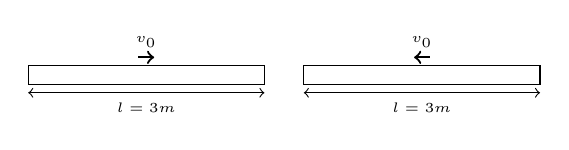
\begin{tikzpicture}
        \draw (0,0) rectangle (3,0.25);
        \draw[<->] (0,-0.1) -- (3,-0.1) node [midway, below] {\tiny $l=3m$};
        \draw[->,thick] (1.4,0.35) -- (1.6,0.35) node [midway, above] {\tiny $v_0$};
        \draw[<->] (3.5,-0.1) -- (6.5,-0.1) node [midway, below] {\tiny $l=3m$};
        \draw[<-,thick] (4.9,0.35) -- (5.1,0.35) node [midway, above] {\tiny $v_0$};
    
        \draw (3.5,0) rectangle (6.5,0.25);
      \end{tikzpicture}
    \end{column}
    \begin{footnotesize}
      \begin{column}{0.49\textwidth}
        $v_0=2.53 \: m/s $; $E= 2\times 10^{11} \: Pa$; $\rho = 7800 \: kg/m^{3}$
      \end{column}
    \end{footnotesize}
  \end{columns}
  \centering
  \begin{tikzpicture}[scale=0.9]
\begin{axis}[xlabel=$time (s)$,ylabel=$\frac{e}{e_{max}}$,ymajorgrids=true,xmajorgrids=true,legend pos=outer north east]%,title={(c) evolution of total energy $e$}]
\addplot[Red,very thick,mark=none,dashed,mark size=3pt] coordinates {(0.0,0.9876543209876545) (1.2090867953958061e-05,0.997530864197531) (2.4181735907916122e-05,1.0) (3.627260386187418e-05,0.9959104938271608) (4.8363471815832244e-05,0.9894000771604939) (6.045433976979031e-05,0.9840934847608025) (7.254520772374836e-05,0.9813625382788388) (8.463607567770642e-05,0.9805725733439128) (9.672694363166447e-05,0.9803534996362381) (0.00010881781158562253,0.9797373358436207) (0.00012090867953958059,0.97855223305006) (0.00013299954749353864,0.9771562700386213) (0.0001450904154474967,0.9759583476912668) (0.00015718128340145475,0.9751165956200767) (0.0001692721513554128,0.9745300840652308) (0.00018136301930937087,0.9740055540525709) (0.00019345388726332892,0.9734177949795755) (0.00020554475521728698,0.9727609779118863) (0.00021763562317124503,0.9721011582864625) (0.0002297264911252031,0.971500815494294) (0.00024181735907916115,0.9709763284318171) (0.0002539082270331192,0.9705033540228475) (0.0002659990949870773,0.9700475116254563) (0.00027808996294103537,0.9695899456257216) (0.00029018083089499345,0.9691327035661251) (0.00030227169884895153,0.96868819213753) (0.0003143625668029096,0.9682659231600772) (0.0003264534347568677,0.9678664411889574) (0.0003385443027108258,0.9674837019503967) (0.00035063517066478387,0.9671110350826551) (0.00036272603861874195,0.9667453037400304) (0.00037481690657270003,0.9663871533998759) (0.0003869077745266581,0.9660386728300239) (0.0003989986424806162,0.9657010208032414) (0.0004110895104345743,0.9653736208998025) (0.00042318037838853236,0.9650548630015646) (0.00043527124634249045,0.9647432582700906) (0.00044736211429644853,0.9644380781342287) (0.0004594529822504066,0.964139187671229) (0.0004715438502043647,0.9638463458344536) (0.0004836347181583228,0.9635583008484584) (0.0004957255861122808,0.9632716356128425) (0.0005078164540662388,0.9629788582366817) (0.0005199073220201969,0.9626650352466273) (0.0005319981899741549,0.9623025558244344) (0.0005440890579281129,0.9618444966372697) (0.000556179925882071,0.9612184911067746) (0.000568270793836029,0.9603246926454502) (0.000580361661789987,0.959042628998641) (0.000592452529743945,0.9572513419900455) };
\addplot[Duck,thin,mark=*,solid,mark size=2pt] coordinates {(0.0,1.0) (1.2090867953958061e-05,0.9799999999999998) (2.4181735907916122e-05,0.97) (3.627260386187418e-05,0.9624999999999999) (4.8363471815832244e-05,0.9562499999999999) (6.045433976979031e-05,0.9507812499999999) (7.254520772374836e-05,0.9458593750000001) (8.463607567770642e-05,0.94134765625) (9.672694363166447e-05,0.937158203125) (0.00010881781158562253,0.9332305908203123) (0.00012090867953958059,0.9295211791992186) (0.00013299954749353864,0.9259972381591796) (0.0001450904154474967,0.9226334762573243) (0.00015718128340145475,0.9194098711013794) (0.0001692721513554128,0.9163102507591249) (0.00018136301930937087,0.9133213311433792) (0.00019345388726332892,0.9104320421814918) (0.00020554475521728698,0.9076330434996636) (0.00021763562317124503,0.9049163683084772) (0.0002297264911252031,0.902275156317046) (0.00024181735907916115,0.8997034499043367) (0.0002539082270331192,0.8971960361519449) (0.0002659990949870773,0.8947483227269913) (0.00027808996294103537,0.8923562391526049) (0.00029018083089499345,0.8900161573950528) (0.00030227169884895153,0.887724827340783) (0.0003143625668029096,0.8854793238875988) (0.0003264534347568677,0.8832770031931295) (0.0003385443027108258,0.8811154662152247) (0.00035063517066478387,0.8789925281119251) (0.00036272603861874195,0.8769061923897169) (0.00037481690657270003,0.8748546289295456) (0.0003869077745266581,0.8728361552026028) (0.0003989986424806162,0.8708492201276435) (0.0004110895104345743,0.8688923901295775) (0.00042318037838853236,0.8669643370432477) (0.00043527124634249045,0.865063827572437) (0.00044736211429644853,0.8631897140664987) (0.0004594529822504066,0.8613409264187486) (0.0004715438502043647,0.8595164649242585) (0.0004836347181583228,0.8577153939617489) (0.0004957255861122808,0.8559368363862708) (0.0005078164540662388,0.8541799685373229) (0.0005199073220201969,0.8524440157818148) (0.0005319981899741549,0.8507282485234637) (0.0005440890579281129,0.8490319786203213) (0.000556179925882071,0.8473545561605471) (0.000568270793836029,0.8456953665535965) (0.000580361661789987,0.8440538278999112) (0.000592452529743945,0.842429388607202) };
\addplot[Orange,very thick,mark=none,densely dotted,mark size=3pt] coordinates {(0.0,0.9873495834618945) (1.1968737974625153e-05,0.9972230792965134) (2.3937475949250306e-05,1.0) (3.590621392387546e-05,0.996543312249306) (4.787495189850061e-05,0.9916724016989357) (5.9843689873125764e-05,0.9886458260672434) (7.181242784775092e-05,0.9877380525503068) (8.378116582237607e-05,0.9876316182265924) (9.574990379700122e-05,0.9872072095327306) (0.00010771864177162638,0.9862586211196859) (0.00011968737974625153,0.9851624959469047) (0.00013165611772087668,0.9842780087964154) (0.00014362485569550183,0.9836648835656183) (0.000155593593670127,0.9831763602119745) (0.00016756233164475214,0.9826698995825812) (0.0001795310696193773,0.9821135512367487) (0.00019149980759400245,0.9815547588976113) (0.0002034685455686276,0.9810419341151472) (0.00021543728354325275,0.9805830603182993) (0.0002274060215178779,0.9801564013202002) (0.00023937475949250306,0.9797401327914591) (0.0002513434974671282,0.979328388660163) (0.00026331223544175336,0.9789272663692082) (0.0002752809734163785,0.9785432962021172) (0.00028724971139100367,0.9781770579069166) (0.0002992184493656288,0.9778246343106916) (0.000311187187340254,0.9774820931955118) (0.0003231559253148791,0.9771479959874065) (0.0003351246632895043,0.9768228205666122) (0.00034709340126412943,0.9765071704950676) (0.0003590621392387546,0.9762007565377634) (0.00037103087721337974,0.97590260746931) (0.0003829996151880049,0.9756117726801273) (0.00039496835316263004,0.9753277223895899) (0.0004069370911372552,0.9750502574593737) (0.00041890582911188035,0.9747792209216646) (0.0004308745670865055,0.9745143288096212) (0.00044284330506113066,0.9742551920745642) (0.0004548120430357558,0.9740013948706343) (0.00046678078101038096,0.9737524481523462) (0.0004787495189850061,0.9735074554284332) (0.0004907182569596313,0.9732642558608436) (0.0005026869949342565,0.9730175918911446) (0.0005146557329088817,0.972755592971648) (0.0005266244708835069,0.9724538550537384) (0.0005385932088581321,0.9720670387858211) (0.0005505619468327574,0.971519585751107) (0.0005625306848073826,0.9706998361345011) (0.0005744994227820078,0.9694646058920318) (0.000586468160756633,0.9676621151764617) };
\addplot[Blue,very thick,mark=none,solid,mark size=3pt] coordinates {(0.0,0.9999999999999998) (2.4181735907916125e-05,0.9999999999999998) (4.836347181583225e-05,0.9999999999999998) (7.254520772374838e-05,0.9999999999999998) (9.67269436316645e-05,0.9999999999999998) (0.00012090867953958063,0.9999999999999998) (0.00014509041544749675,1.0) (0.0001692721513554129,0.9999999999999998) (0.000193453887263329,0.9999999999999998) (0.00021763562317124512,0.9999999999999998) (0.00024181735907916123,0.9999999999999998) (0.00026599909498707734,0.9999999999999997) (0.00029018083089499345,0.9999999999999997) (0.00031436256680290956,0.9999999999999997) (0.0003385443027108257,0.9999999999999997) (0.0003627260386187418,0.9999999999999997) (0.0003869077745266579,0.9999999999999997) (0.000411089510434574,0.9999999999999997) (0.0004352712463424901,0.9999999999999994) (0.00045945298225040623,0.9999999999999997) (0.00048363471815832235,0.9999999999999994) (0.0005078164540662385,0.9999999999999992) (0.0005319981899741547,0.9999999999999992) (0.0005561799258820708,0.9999999999999992) (0.000580361661789987,0.9999999999999992) (0.0006045433976979032,0.9999999999999992) };
\addplot[Purple,very thick,mark=|,solid,mark size=3pt] coordinates {(0.0,1.0) (1.1968737974625153e-05,0.9849999999999999) (2.3937475949250306e-05,0.9782812499999997) (3.590621392387546e-05,0.9728686523437499) (4.787495189850061e-05,0.9685175323486328) (5.9843689873125764e-05,0.9646764224767683) (7.181242784775092e-05,0.9612245353125033) (8.378116582237607e-05,0.9580584139595156) (9.574990379700122e-05,0.9551170218177228) (0.00010771864177162638,0.9523583400291113) (0.00011968737974625153,0.9497518470633621) (0.00013165611772087668,0.9472747764554426) (0.00014362485569550183,0.9449095127565772) (0.000155593593670127,0.942642119512832) (0.00016756233164475214,0.9404613389338139) (0.0001795310696193773,0.9383579222991295) (0.00019149980759400245,0.9363241607011475) (0.0002034685455686276,0.9343535480062032) (0.00021543728354325275,0.9324405332414724) (0.0002274060215178779,0.9305803349197901) (0.00023937475949250306,0.928768799378865) (0.0002513434974671282,0.9270022910038743) (0.00026331223544175336,0.9252776059761404) (0.0002752809734163785,0.9235919036615065) (0.00028724971139100367,0.9219426514179895) (0.0002992184493656288,0.9203275797465361) (0.000311187187340254,0.9187446455091373) (0.0003231559253148791,0.9171920015078542) (0.0003351246632895043,0.915667971129286) (0.00034709340126412943,0.914171027059833) (0.0003590621392387546,0.9126997733000616) (0.00037103087721337974,0.9112529298736883) (0.0003829996151880049,0.9098293197534216) (0.00039496835316263004,0.9084278576229242) (0.0004069370911372552,0.9070475401691336) (0.00041890582911188035,0.9056874376575983) (0.0004308745670865055,0.9043466865894064) (0.00044284330506113066,0.9030244832746345) (0.0004548120430357558,0.9017200781862146) (0.00046678078101038096,0.9004327709813899) (0.0004787495189850061,0.8991619060967203) (0.0004907182569596313,0.897906868837865) (0.0005026869949342565,0.8966670818978505) (0.0005146557329088817,0.8954420022477787) (0.0005266244708835069,0.8942311183524017) (0.0005385932088581321,0.8930339476700012) (0.0005505619468327574,0.8918500344018717) (0.0005625306848073826,0.8906789474616031) (0.0005744994227820078,0.8895202786384733) (0.000586468160756633,0.8883736409327396) (0.0005984368987312582,0.8872386670435604) };
\addplot[Green,thick,mark=x,only marks,mark size=3pt] coordinates {(0.0,1.0) (2.3937475949250306e-05,0.9999999999999997) (4.787495189850061e-05,0.9999999999999998) (7.181242784775092e-05,0.9999999999999998) (9.574990379700122e-05,0.9999999999999998) (0.00011968737974625153,0.9999999999999998) (0.00014362485569550183,0.9999999999999998) (0.00016756233164475214,0.9999999999999997) (0.00019149980759400245,0.9999999999999997) (0.00021543728354325275,0.9999999999999994) (0.00023937475949250306,0.9999999999999994) (0.00026331223544175336,0.9999999999999992) (0.00028724971139100367,0.999999999999999) (0.000311187187340254,0.999999999999999) (0.0003351246632895043,0.999999999999999) (0.0003590621392387546,0.999999999999999) (0.0003829996151880049,0.999999999999999) (0.0004069370911372552,0.999999999999999) (0.0004308745670865055,0.999999999999999) (0.0004548120430357558,0.999999999999999) (0.0004787495189850061,0.9999999999999989) (0.0005026869949342564,0.999999999999999) (0.0005266244708835067,0.999999999999999) (0.000550561946832757,0.9999999999999989) (0.0005744994227820073,0.9999999999999989) (0.0005984368987312576,0.999999999999999) };
\addplot[black,thin,mark=none,solid,mark size=3pt] coordinates {(0.0,1.0) (1e-08,1.0) };
\legend{usl 1ppc,usl-pic 1ppc,usl 2ppc,dgmpm 1ppc,dgmpm 2ppc,dgmpm 2ppc (RK2),exact}
\end{axis}
\end{tikzpicture}
%%% Local Variables:
%%% mode: latex
%%% TeX-master: "../../mainManuscript"
%%% End:

  \footnoteCite{Wang}
\end{frame}

\begin{frame}{Riemann problem in a one-dimensional elastic-plastic medium \cite{Thomas_EP}}
  \vskip 5pt
  \begin{columns}
    \begin{column}{0.49\textwidth}
      Plane wave state: $\tens{\eps}=\eps \vect{e}_1 \otimes \vect{e}_1$ % \sigma_{22},\sigma_{33}\neq 0
    \end{column}
    \begin{footnotesize}
      \begin{column}{0.49\textwidth}
        Isotropic linear hardening of modulus $C=10^9 \:Pa$ \\
        $v_0$ leading to plastic flow \\
        %% EP or Elastic Riemann solver coupled to a radial return algorithm \cite{Simo}
      \end{column}
    \end{footnotesize}
  \end{columns}
  \centering
  \begin{tikzpicture}[scale=.7]
\begin{groupplot}[group style={group size=2 by 2,
ylabels at=edge left,horizontal sep=11.ex,
vertical sep=4ex,xticklabels at=edge bottom,xlabels at=edge bottom},
ymajorgrids=true,xmajorgrids=true,enlargelimits=0,xmin=0.,xmax=6.,xlabel=$x (m)$,
axis on top,scale only axis,width=0.48\linewidth,legend pos=outer north east
]
\nextgroupplot[title={\footnotesize Incident waves -- Stress},ymin=-1.35e9,ymax=56579516.10614197,,xlabel=$x (m)$,ylabel=$\sigma \: (Pa)$]
\addplot[Red,dashed,mark=none,very thick,mark size=3pt,mark repeat=2] coordinates{(0.0,-8433215.03790355) (0.12244897959183673,-31379937.150059074) (0.24489795918367346,-73325965.87671247) (0.36734693877551017,-147815909.35881704) (0.4897959183673469,-264501011.32373637) (0.6122448979591837,-419797360.6339785) (0.7346938775510203,-586994803.1537646) (0.8571428571428571,-715242874.2277462) (0.9795918367346939,-804731796.1198385) (1.1020408163265305,-919403784.9173691) (1.2244897959183674,-1063504114.033879) (1.346938775510204,-1209904754.949398) (1.4693877551020407,-1304654513.0867395) (1.5918367346938775,-1291382612.5749428) (1.7142857142857142,-1218226204.6353252) (1.836734693877551,-1185455835.0777807) (1.9591836734693877,-1232745182.470082) (2.0816326530612246,-1261396271.0817113) (2.204081632653061,-1270103667.4391637) (2.326530612244898,-1227250869.598082) (2.4489795918367347,-1235273389.504192) (2.571428571428571,-1229787858.686364) (2.693877551020408,-1255621316.42765) (2.816326530612245,-1241442333.7811728) (2.9387755102040813,-1239848703.7218106) (3.061224489795918,-1239848703.7218091) (3.183673469387755,-1241442333.781176) (3.306122448979592,-1255621316.4276485) (3.4285714285714284,-1229787858.6863654) (3.5510204081632653,-1235273389.5041904) (3.673469387755102,-1227250869.598084) (3.7959183673469385,-1270103667.439164) (3.9183673469387754,-1261396271.081712) (4.040816326530612,-1232745182.4700806) (4.163265306122449,-1185455835.0777805) (4.285714285714286,-1218226204.6353254) (4.408163265306122,-1291382612.5749435) (4.530612244897959,-1304654513.0867395) (4.653061224489796,-1209904754.9493968) (4.775510204081632,-1063504114.033878) (4.8979591836734695,-919403784.917369) (5.020408163265306,-804731796.1198374) (5.142857142857142,-715242874.2277458) (5.26530612244898,-586994803.1537648) (5.387755102040816,-419797360.63397753) (5.5102040816326525,-264501011.3237358) (5.63265306122449,-147815909.35881624) (5.755102040816326,-73325965.8767119) (5.877551020408163,-31379937.150058918) (6.0,-8433215.037903389) };
\addplot[Blue,solid,mark=+,thick,mark size=3pt,mark repeat=2] coordinates{(0.0,-3.2561158711216654e-07) (0.12244897959183673,-6.54162606232603e-22) (0.24489795918367346,0.0) (0.36734693877551017,3.2561158711216643e-07) (0.4897959183673469,-4.884173806682499e-07) (0.6122448979591837,-710637837.2357953) (0.7346938775510203,-747893724.781927) (0.8571428571428571,-827829409.8631966) (0.9795918367346939,-936780409.853217) (1.1020408163265305,-1054073198.2499647) (1.2244897959183674,-1144128439.1849532) (1.346938775510204,-1207925723.6670742) (1.4693877551020407,-1232372577.7948787) (1.5918367346938775,-1254253728.274747) (1.7142857142857142,-1243570946.3490026) (1.836734693877551,-1268139963.2569304) (1.9591836734693877,-1248035262.8872383) (2.0816326530612246,-1268992337.693115) (2.204081632653061,-1251285653.8729925) (2.326530612244898,-1266352346.5241969) (2.4489795918367347,-1253527311.8706975) (2.571428571428571,-1264419055.233534) (2.693877551020408,-1255474245.0991223) (2.816326530612245,-1261578869.0693417) (2.9387755102040813,-1258168698.6750736) (3.061224489795918,-1258168698.6750731) (3.183673469387755,-1261578869.069342) (3.306122448979592,-1255474245.0991209) (3.4285714285714284,-1264419055.233534) (3.5510204081632653,-1253527311.870696) (3.673469387755102,-1266352346.5241973) (3.7959183673469385,-1251285653.8729923) (3.9183673469387754,-1268992337.6931143) (4.040816326530612,-1248035262.8872375) (4.163265306122449,-1268139963.2569308) (4.285714285714286,-1243570946.3490026) (4.408163265306122,-1254253728.2747467) (4.530612244897959,-1232372577.7948787) (4.653061224489796,-1207925723.6670735) (4.775510204081632,-1144128439.1849532) (4.8979591836734695,-1054073198.2499645) (5.020408163265306,-936780409.853217) (5.142857142857142,-827829409.8631967) (5.26530612244898,-747893724.7819276) (5.387755102040816,-710637837.2357956) (5.5102040816326525,-4.884173806682498e-07) (5.63265306122449,0.0) (5.755102040816326,-4.884173806682498e-07) (5.877551020408163,0.0) (6.0,-4.884173806682498e-07) };
\addplot[Orange,solid,mark=o,very thick,mark size=2pt,mark repeat=2] coordinates{(0.0,0.0) (0.12244897959183673,0.0) (0.24489795918367346,0.0) (0.36734693877551017,0.0) (0.4897959183673469,0.0) (0.6122448979591837,-700099961.461325) (0.7346938775510203,-702215400.6707044) (0.8571428571428571,-720845446.6905135) (0.9795918367346939,-807249777.2239016) (1.1020408163265305,-1021817726.088786) (1.2244897959183674,-1257135415.8766613) (1.346938775510204,-1201909815.2742617) (1.4693877551020407,-1284541316.0967622) (1.5918367346938775,-1197762497.5853782) (1.7142857142857142,-1280230396.1356874) (1.836734693877551,-1230639248.475009) (1.9591836734693877,-1232614670.2907715) (2.0816326530612246,-1296340561.1434355) (2.204081632653061,-1163180742.3691304) (2.326530612244898,-1344085453.2920678) (2.4489795918367347,-1125286993.986051) (2.571428571428571,-1354573027.5700727) (2.693877551020408,-1144440690.6862848) (2.816326530612245,-1331966839.3238678) (2.9387755102040813,-1234245710.8866477) (3.061224489795918,-1234245710.8866642) (3.183673469387755,-1331966839.3238637) (3.306122448979592,-1144440690.6862931) (3.4285714285714284,-1354573027.570076) (3.5510204081632653,-1125286993.9860492) (3.673469387755102,-1344085453.2920709) (3.7959183673469385,-1163180742.369132) (3.9183673469387754,-1296340561.143439) (4.040816326530612,-1232614670.2907667) (4.163265306122449,-1230639248.4750104) (4.285714285714286,-1280230396.1356888) (4.408163265306122,-1197762497.5853772) (4.530612244897959,-1284541316.0967634) (4.653061224489796,-1201909815.2742698) (4.775510204081632,-1257135415.8766532) (4.8979591836734695,-1021817726.0887933) (5.020408163265306,-807249777.2238963) (5.142857142857142,-720845446.6905184) (5.26530612244898,-702215400.6706979) (5.387755102040816,-700099961.4613259) (5.5102040816326525,0.0) (5.63265306122449,0.0) (5.755102040816326,0.0) (5.877551020408163,0.0) (6.0,0.0) };
\addplot[Purple,solid,mark=x,thick,mark size=3pt,mark repeat=2] coordinates{(0.0,0.0) (0.12244897959183673,0.0) (0.24489795918367346,0.0) (0.36734693877551017,0.0) (0.4897959183673469,0.0) (0.6122448979591837,-700149009.8511133) (0.7346938775510203,-702792255.866507) (0.8571428571428571,-725326867.326901) (0.9795918367346939,-850156660.8530495) (1.1020408163265305,-1109984935.9712873) (1.2244897959183674,-1250258832.4370122) (1.346938775510204,-1260471082.9558206) (1.4693877551020407,-1260981625.9873586) (1.5918367346938775,-1261003693.8957453) (1.7142857142857142,-1261004546.9659622) (1.836734693877551,-1261004575.4299965) (1.9591836734693877,-1261004576.2405941) (2.0816326530612246,-1261004576.260158) (2.204081632653061,-1261004576.2605524) (2.326530612244898,-1261004576.260559) (2.4489795918367347,-1261004576.260559) (2.571428571428571,-1261004576.260559) (2.693877551020408,-1261004576.260559) (2.816326530612245,-1261004576.2605588) (2.9387755102040813,-1261004576.2605588) (3.061224489795918,-1261004576.260559) (3.183673469387755,-1261004576.2605588) (3.306122448979592,-1261004576.2605588) (3.4285714285714284,-1261004576.2605588) (3.5510204081632653,-1261004576.2605588) (3.673469387755102,-1261004576.2605588) (3.7959183673469385,-1261004576.260553) (3.9183673469387754,-1261004576.2601585) (4.040816326530612,-1261004576.2405944) (4.163265306122449,-1261004575.4299967) (4.285714285714286,-1261004546.9659626) (4.408163265306122,-1261003693.895745) (4.530612244897959,-1260981625.987358) (4.653061224489796,-1260471082.955823) (4.775510204081632,-1250258832.4370096) (4.8979591836734695,-1109984935.971287) (5.020408163265306,-850156660.8530501) (5.142857142857142,-725326867.326901) (5.26530612244898,-702792255.866507) (5.387755102040816,-700149009.8511133) (5.5102040816326525,0.0) (5.63265306122449,0.0) (5.755102040816326,0.0) (5.877551020408163,0.0) (6.0,0.0) };
\addplot[black,solid,mark=none,thin,mark size=3pt,mark repeat=2] coordinates{(0.0,-0.0) (0.12244897959183673,-0.0) (0.24489795918367346,-0.0) (0.36734693877551017,-0.0) (0.4897959183673469,-0.0) (0.6122448979591837,-700000000.0) (0.7346938775510203,-700000000.0) (0.8571428571428571,-700000000.0) (0.9795918367346939,-700000000.0) (1.1020408163265305,-1261004576.260559) (1.2244897959183674,-1261004576.260559) (1.346938775510204,-1261004576.260559) (1.4693877551020407,-1261004576.260559) (1.5918367346938775,-1261004576.260559) (1.7142857142857142,-1261004576.260559) (1.836734693877551,-1261004576.260559) (1.9591836734693877,-1261004576.260559) (2.0816326530612246,-1261004576.260559) (2.204081632653061,-1261004576.260559) (2.326530612244898,-1261004576.260559) (2.4489795918367347,-1261004576.260559) (2.571428571428571,-1261004576.260559) (2.693877551020408,-1261004576.260559) (2.816326530612245,-1261004576.260559) (2.9387755102040813,-1261004576.260559) (3.061224489795918,-1261004576.260559) (3.183673469387755,-1261004576.260559) (3.306122448979592,-1261004576.260559) (3.4285714285714284,-1261004576.260559) (3.5510204081632653,-1261004576.260559) (3.673469387755102,-1261004576.260559) (3.7959183673469385,-1261004576.260559) (3.9183673469387754,-1261004576.260559) (4.040816326530612,-1261004576.260559) (4.163265306122449,-1261004576.260559) (4.285714285714286,-1261004576.260559) (4.408163265306122,-1261004576.260559) (4.530612244897959,-1261004576.260559) (4.653061224489796,-1261004576.260559) (4.775510204081632,-1261004576.260559) (4.8979591836734695,-1261004576.260559) (5.020408163265306,-700000000.0) (5.142857142857142,-700000000.0) (5.26530612244898,-700000000.0) (5.387755102040816,-700000000.0) (5.5102040816326525,-0.0) (5.63265306122449,-0.0) (5.755102040816326,-0.0) (5.877551020408163,-0.0) (6.0,-0.0) };

\nextgroupplot[title={\footnotesize Incident waves -- Plastic strain},ymin=-0.0034,ymax=0.0,xlabel=$x \:(m)$,ylabel=$\eps^p$]
\addplot[Red,dashed,mark=none,very thick,mark size=3pt,mark repeat=2] coordinates{(0.0,0.0) (0.12244897959183673,0.0) (0.24489795918367346,0.0) (0.36734693877551017,0.0) (0.4897959183673469,0.0) (0.6122448979591837,0.0) (0.7346938775510203,0.0) (0.8571428571428571,-5.5177825258810104e-05) (0.9795918367346939,-0.0003791196239632164) (1.1020408163265305,-0.0007942218458547296) (1.2244897959183674,-0.0013158519965027296) (1.346938775510204,-0.0018458090676901286) (1.4693877551020407,-0.002188794617508559) (1.5918367346938775,-0.002229697455331896) (1.7142857142857142,-0.002258121963594508) (1.836734693877551,-0.002271799079674154) (1.9591836734693877,-0.002320613632318322) (2.0816326530612246,-0.002313868472160546) (2.204081632653061,-0.0024020122032007017) (2.326530612244898,-0.0023588630990294623) (2.4489795918367347,-0.0025433455597807667) (2.571428571428571,-0.002385435935351422) (2.693877551020408,-0.0027693350417516906) (2.816326530612245,-0.0024065265204776445) (2.9387755102040813,-0.0032250612006492966) (3.061224489795918,-0.0032250612006492524) (3.183673469387755,-0.002406526520477666) (3.306122448979592,-0.0027693350417516823) (3.4285714285714284,-0.0023854359353514295) (3.5510204081632653,-0.0025433455597807628) (3.673469387755102,-0.002358863099029464) (3.7959183673469385,-0.0024020122032006983) (3.9183673469387754,-0.0023138684721605448) (4.040816326530612,-0.002320613632318319) (4.163265306122449,-0.0022717990796741546) (4.285714285714286,-0.0022581219635945077) (4.408163265306122,-0.0022296974553318956) (4.530612244897959,-0.0021887946175085595) (4.653061224489796,-0.001845809067690125) (4.775510204081632,-0.0013158519965027254) (4.8979591836734695,-0.0007942218458547295) (5.020408163265306,-0.0003791196239632123) (5.142857142857142,-5.5177825258808404e-05) (5.26530612244898,0.0) (5.387755102040816,0.0) (5.5102040816326525,0.0) (5.63265306122449,0.0) (5.755102040816326,0.0) (5.877551020408163,0.0) (6.0,0.0) };
\addplot[Blue,solid,mark=+,thick,mark size=3pt,mark repeat=2] coordinates{(0.0,0.0) (0.12244897959183673,0.0) (0.24489795918367346,0.0) (0.36734693877551017,0.0) (0.4897959183673469,0.0) (0.6122448979591837,-3.850800809337606e-05) (0.7346938775510203,-0.00017337094943683953) (0.8571428571428571,-0.00046273089543238553) (0.9795918367346939,-0.000857123655577256) (1.1020408163265305,-0.0012817129348415013) (1.2244897959183674,-0.0016077047572306) (1.346938775510204,-0.0018386451535459692) (1.4693877551020407,-0.0019271405531036338) (1.5918367346938775,-0.002006348337646142) (1.7142857142857142,-0.002018045326373221) (1.836734693877551,-0.002056615251608797) (1.9591836734693877,-0.0020613216365693464) (2.0816326530612246,-0.002064203896841495) (2.204081632653061,-0.0020644266901542695) (2.326530612244898,-0.0020621094945296272) (2.4489795918367347,-0.002062767607181189) (2.571428571428571,-0.002061489252343496) (2.693877551020408,-0.0020573197208032658) (2.816326530612245,-0.0020502799029179) (2.9387755102040813,-0.0020377776694292327) (3.061224489795918,-0.0020377776694292327) (3.183673469387755,-0.002050279902917899) (3.306122448979592,-0.002057319720803265) (3.4285714285714284,-0.0020614892523434956) (3.5510204081632653,-0.0020627676071811878) (3.673469387755102,-0.0020621094945296285) (3.7959183673469385,-0.0020644266901542695) (3.9183673469387754,-0.0020642038968414953) (4.040816326530612,-0.0020613216365693477) (4.163265306122449,-0.002056615251608799) (4.285714285714286,-0.0020180453263732205) (4.408163265306122,-0.0020063483376461405) (4.530612244897959,-0.0019271405531036334) (4.653061224489796,-0.0018386451535459673) (4.775510204081632,-0.0016077047572305996) (4.8979591836734695,-0.0012817129348415002) (5.020408163265306,-0.0008571236555772557) (5.142857142857142,-0.000462730895432386) (5.26530612244898,-0.0001733709494368422) (5.387755102040816,-3.850800809337776e-05) (5.5102040816326525,0.0) (5.63265306122449,0.0) (5.755102040816326,0.0) (5.877551020408163,0.0) (6.0,0.0) };
\addplot[Orange,solid,mark=o,very thick,mark size=2pt,mark repeat=2] coordinates{(0.0,0.0) (0.12244897959183673,0.0) (0.24489795918367346,0.0) (0.36734693877551017,0.0) (0.4897959183673469,0.0) (0.6122448979591837,-3.6185144371068533e-07) (0.7346938775510203,-8.019549939201378e-06) (0.8571428571428571,-7.545863055389513e-05) (0.9795918367346939,-0.00038823448768833166) (1.1020408163265305,-0.0011649510446652884) (1.2244897959183674,-0.0020167797859788647) (1.346938775510204,-0.002107399619958115) (1.4693877551020407,-0.002131770374563102) (1.5918367346938775,-0.0021403574192086572) (1.7142857142857142,-0.0021224712498380525) (1.836734693877551,-0.0021223153729543927) (1.9591836734693877,-0.002051517588290279) (2.0816326530612246,-0.00215869886386764) (2.204081632653061,-0.00229323761080671) (2.326530612244898,-0.002383730340592019) (2.4489795918367347,-0.002422023782426279) (2.571428571428571,-0.0024301527006305407) (2.693877551020408,-0.0023776240406298606) (2.816326530612245,-0.0022924966391795762) (2.9387755102040813,-0.002209718054457858) (3.061224489795918,-0.002209718054457853) (3.183673469387755,-0.00229249663917957) (3.306122448979592,-0.002377624040629834) (3.4285714285714284,-0.0024301527006305133) (3.5510204081632653,-0.0024220237824262893) (3.673469387755102,-0.0023837303405920274) (3.7959183673469385,-0.0022932376108067225) (3.9183673469387754,-0.002158698863867652) (4.040816326530612,-0.0020515175882902612) (4.163265306122449,-0.00212231537295439) (4.285714285714286,-0.002122471249838043) (4.408163265306122,-0.002140357419208655) (4.530612244897959,-0.0021317703745630944) (4.653061224489796,-0.0021073996199581038) (4.775510204081632,-0.002016779785978835) (4.8979591836734695,-0.0011649510446653149) (5.020408163265306,-0.00038823448768831226) (5.142857142857142,-7.54586305539126e-05) (5.26530612244898,-8.019549939178096e-06) (5.387755102040816,-3.6185144371335306e-07) (5.5102040816326525,0.0) (5.63265306122449,0.0) (5.755102040816326,0.0) (5.877551020408163,0.0) (6.0,0.0) };
\addplot[Purple,solid,mark=x,thick,mark size=3pt,mark repeat=2] coordinates{(0.0,0.0) (0.12244897959183673,0.0) (0.24489795918367346,0.0) (0.36734693877551017,0.0) (0.4897959183673469,0.0) (0.6122448979591837,-5.394021759754931e-07) (0.7346938775510203,-1.010771354391672e-05) (0.8571428571428571,-9.168096769918878e-05) (0.9795918367346939,-0.0005435535234499527) (1.1020408163265305,-0.0014841083655069223) (1.2244897959183674,-0.001991887176242578) (1.346938775510204,-0.002028854598935097) (1.4693877551020407,-0.0020307027185062754) (1.5918367346938775,-0.002030782602337539) (1.7142857142857142,-0.0020307856903745234) (1.836734693877551,-0.002030785793411752) (1.9591836734693877,-0.002030785796346042) (2.0816326530612246,-0.002030785796416862) (2.204081632653061,-0.002030785796418289) (2.326530612244898,-0.0020307857964183135) (2.4489795918367347,-0.0020307857964183135) (2.571428571428571,-0.0020307857964183135) (2.693877551020408,-0.0020307857964183135) (2.816326530612245,-0.0020307857964183135) (2.9387755102040813,-0.0020307857964183135) (3.061224489795918,-0.0020307857964183135) (3.183673469387755,-0.0020307857964183135) (3.306122448979592,-0.0020307857964183126) (3.4285714285714284,-0.0020307857964183135) (3.5510204081632653,-0.0020307857964183126) (3.673469387755102,-0.0020307857964183126) (3.7959183673469385,-0.002030785796418291) (3.9183673469387754,-0.0020307857964168632) (4.040816326530612,-0.0020307857963460427) (4.163265306122449,-0.0020307857934117523) (4.285714285714286,-0.002030785690374525) (4.408163265306122,-0.0020307826023375384) (4.530612244897959,-0.0020307027185062733) (4.653061224489796,-0.002028854598935106) (4.775510204081632,-0.0019918871762425686) (4.8979591836734695,-0.0014841083655069208) (5.020408163265306,-0.0005435535234499549) (5.142857142857142,-9.168096769918878e-05) (5.26530612244898,-1.010771354391672e-05) (5.387755102040816,-5.394021759754931e-07) (5.5102040816326525,0.0) (5.63265306122449,0.0) (5.755102040816326,0.0) (5.877551020408163,0.0) (6.0,0.0) };
\addplot[black,solid,mark=none,thin,mark size=3pt,mark repeat=2] coordinates{(0.0,-0.0) (0.12244897959183673,-0.0) (0.24489795918367346,-0.0) (0.36734693877551017,-0.0) (0.4897959183673469,-0.0) (0.6122448979591837,-0.0) (0.7346938775510203,-0.0) (0.8571428571428571,-0.0) (0.9795918367346939,-0.0) (1.1020408163265305,-0.002030785796418313) (1.2244897959183674,-0.002030785796418313) (1.346938775510204,-0.002030785796418313) (1.4693877551020407,-0.002030785796418313) (1.5918367346938775,-0.002030785796418313) (1.7142857142857142,-0.002030785796418313) (1.836734693877551,-0.002030785796418313) (1.9591836734693877,-0.002030785796418313) (2.0816326530612246,-0.002030785796418313) (2.204081632653061,-0.002030785796418313) (2.326530612244898,-0.002030785796418313) (2.4489795918367347,-0.002030785796418313) (2.571428571428571,-0.002030785796418313) (2.693877551020408,-0.002030785796418313) (2.816326530612245,-0.002030785796418313) (2.9387755102040813,-0.002030785796418313) (3.061224489795918,-0.002030785796418313) (3.183673469387755,-0.002030785796418313) (3.306122448979592,-0.002030785796418313) (3.4285714285714284,-0.002030785796418313) (3.5510204081632653,-0.002030785796418313) (3.673469387755102,-0.002030785796418313) (3.7959183673469385,-0.002030785796418313) (3.9183673469387754,-0.002030785796418313) (4.040816326530612,-0.002030785796418313) (4.163265306122449,-0.002030785796418313) (4.285714285714286,-0.002030785796418313) (4.408163265306122,-0.002030785796418313) (4.530612244897959,-0.002030785796418313) (4.653061224489796,-0.002030785796418313) (4.775510204081632,-0.002030785796418313) (4.8979591836734695,-0.002030785796418313) (5.020408163265306,-0.0) (5.142857142857142,-0.0) (5.26530612244898,-0.0) (5.387755102040816,-0.0) (5.5102040816326525,-0.0) (5.63265306122449,-0.0) (5.755102040816326,-0.0) (5.877551020408163,-0.0) (6.0,-0.0) };
\addlegendentry{mpm}
\addlegendentry{dgmpm}
\addlegendentry{fem}
\addlegendentry{fvm (SB)}
\addlegendentry{exact}

\end{groupplot}
\end{tikzpicture}
%%% Local Variables:
%%% mode: latex
%%% TeX-master: "../../presentation"
%%% End:

  \footnoteCite{Thomas_EP}
\end{frame}

\begin{frame}{Riemann problem in a one-dimensional elastic-plastic medium \cite{Thomas_EP}}
  \vskip 5pt
  \begin{columns}
    \begin{column}{0.49\textwidth}
      Plane wave state: $\tens{\eps}=\eps \vect{e}_1 \otimes \vect{e}_1$ % \sigma_{22},\sigma_{33}\neq 0
    \end{column}
    \begin{footnotesize}
      \begin{column}{0.49\textwidth}
        Isotropic linear hardening of modulus $C=10^9 \:Pa$ \\
        $v_0$ leading to plastic flow \\
        %% EP or Elastic Riemann solver coupled to a radial return algorithm \cite{Simo}
      \end{column}
    \end{footnotesize}
  \end{columns}
    \centering
    \begin{tikzpicture}[scale=.6]
\begin{groupplot}[group style={group size=2 by 2,
ylabels at=edge left, yticklabels at=edge left,horizontal sep=2.ex,
vertical sep=4ex,xticklabels at=edge bottom,xlabels at=edge bottom},
ymajorgrids=true,xmajorgrids=true,enlargelimits=0,xmin=0.,xmax=6.,xlabel=$x (m)$,
axis on top,scale only axis,width=0.48\linewidth,legend pos=outer north east
]

\nextgroupplot[title={Incident waves -- Plastic strain},ymin=-0.0034,ymax=0.0,xlabel=$x \:(m)$,ylabel=$\eps^p$]
\addplot[Red,dashed,mark=none,very thick,mark size=3pt,mark repeat=2] coordinates{(0.0,0.0) (0.12244897959183673,0.0) (0.24489795918367346,0.0) (0.36734693877551017,0.0) (0.4897959183673469,0.0) (0.6122448979591837,0.0) (0.7346938775510203,0.0) (0.8571428571428571,-5.5177825258810104e-05) (0.9795918367346939,-0.0003791196239632164) (1.1020408163265305,-0.0007942218458547296) (1.2244897959183674,-0.0013158519965027296) (1.346938775510204,-0.0018458090676901286) (1.4693877551020407,-0.002188794617508559) (1.5918367346938775,-0.002229697455331896) (1.7142857142857142,-0.002258121963594508) (1.836734693877551,-0.002271799079674154) (1.9591836734693877,-0.002320613632318322) (2.0816326530612246,-0.002313868472160546) (2.204081632653061,-0.0024020122032007017) (2.326530612244898,-0.0023588630990294623) (2.4489795918367347,-0.0025433455597807667) (2.571428571428571,-0.002385435935351422) (2.693877551020408,-0.0027693350417516906) (2.816326530612245,-0.0024065265204776445) (2.9387755102040813,-0.0032250612006492966) (3.061224489795918,-0.0032250612006492524) (3.183673469387755,-0.002406526520477666) (3.306122448979592,-0.0027693350417516823) (3.4285714285714284,-0.0023854359353514295) (3.5510204081632653,-0.0025433455597807628) (3.673469387755102,-0.002358863099029464) (3.7959183673469385,-0.0024020122032006983) (3.9183673469387754,-0.0023138684721605448) (4.040816326530612,-0.002320613632318319) (4.163265306122449,-0.0022717990796741546) (4.285714285714286,-0.0022581219635945077) (4.408163265306122,-0.0022296974553318956) (4.530612244897959,-0.0021887946175085595) (4.653061224489796,-0.001845809067690125) (4.775510204081632,-0.0013158519965027254) (4.8979591836734695,-0.0007942218458547295) (5.020408163265306,-0.0003791196239632123) (5.142857142857142,-5.5177825258808404e-05) (5.26530612244898,0.0) (5.387755102040816,0.0) (5.5102040816326525,0.0) (5.63265306122449,0.0) (5.755102040816326,0.0) (5.877551020408163,0.0) (6.0,0.0) };
\addplot[Blue,solid,mark=+,thick,mark size=3pt,mark repeat=2] coordinates{(0.0,0.0) (0.12244897959183673,0.0) (0.24489795918367346,0.0) (0.36734693877551017,0.0) (0.4897959183673469,0.0) (0.6122448979591837,-3.850800809337606e-05) (0.7346938775510203,-0.00017337094943683953) (0.8571428571428571,-0.00046273089543238553) (0.9795918367346939,-0.000857123655577256) (1.1020408163265305,-0.0012817129348415013) (1.2244897959183674,-0.0016077047572306) (1.346938775510204,-0.0018386451535459692) (1.4693877551020407,-0.0019271405531036338) (1.5918367346938775,-0.002006348337646142) (1.7142857142857142,-0.002018045326373221) (1.836734693877551,-0.002056615251608797) (1.9591836734693877,-0.0020613216365693464) (2.0816326530612246,-0.002064203896841495) (2.204081632653061,-0.0020644266901542695) (2.326530612244898,-0.0020621094945296272) (2.4489795918367347,-0.002062767607181189) (2.571428571428571,-0.002061489252343496) (2.693877551020408,-0.0020573197208032658) (2.816326530612245,-0.0020502799029179) (2.9387755102040813,-0.0020377776694292327) (3.061224489795918,-0.0020377776694292327) (3.183673469387755,-0.002050279902917899) (3.306122448979592,-0.002057319720803265) (3.4285714285714284,-0.0020614892523434956) (3.5510204081632653,-0.0020627676071811878) (3.673469387755102,-0.0020621094945296285) (3.7959183673469385,-0.0020644266901542695) (3.9183673469387754,-0.0020642038968414953) (4.040816326530612,-0.0020613216365693477) (4.163265306122449,-0.002056615251608799) (4.285714285714286,-0.0020180453263732205) (4.408163265306122,-0.0020063483376461405) (4.530612244897959,-0.0019271405531036334) (4.653061224489796,-0.0018386451535459673) (4.775510204081632,-0.0016077047572305996) (4.8979591836734695,-0.0012817129348415002) (5.020408163265306,-0.0008571236555772557) (5.142857142857142,-0.000462730895432386) (5.26530612244898,-0.0001733709494368422) (5.387755102040816,-3.850800809337776e-05) (5.5102040816326525,0.0) (5.63265306122449,0.0) (5.755102040816326,0.0) (5.877551020408163,0.0) (6.0,0.0) };
\addplot[Orange,solid,mark=o,very thick,mark size=2pt,mark repeat=2] coordinates{(0.0,0.0) (0.12244897959183673,0.0) (0.24489795918367346,0.0) (0.36734693877551017,0.0) (0.4897959183673469,0.0) (0.6122448979591837,-3.6185144371068533e-07) (0.7346938775510203,-8.019549939201378e-06) (0.8571428571428571,-7.545863055389513e-05) (0.9795918367346939,-0.00038823448768833166) (1.1020408163265305,-0.0011649510446652884) (1.2244897959183674,-0.0020167797859788647) (1.346938775510204,-0.002107399619958115) (1.4693877551020407,-0.002131770374563102) (1.5918367346938775,-0.0021403574192086572) (1.7142857142857142,-0.0021224712498380525) (1.836734693877551,-0.0021223153729543927) (1.9591836734693877,-0.002051517588290279) (2.0816326530612246,-0.00215869886386764) (2.204081632653061,-0.00229323761080671) (2.326530612244898,-0.002383730340592019) (2.4489795918367347,-0.002422023782426279) (2.571428571428571,-0.0024301527006305407) (2.693877551020408,-0.0023776240406298606) (2.816326530612245,-0.0022924966391795762) (2.9387755102040813,-0.002209718054457858) (3.061224489795918,-0.002209718054457853) (3.183673469387755,-0.00229249663917957) (3.306122448979592,-0.002377624040629834) (3.4285714285714284,-0.0024301527006305133) (3.5510204081632653,-0.0024220237824262893) (3.673469387755102,-0.0023837303405920274) (3.7959183673469385,-0.0022932376108067225) (3.9183673469387754,-0.002158698863867652) (4.040816326530612,-0.0020515175882902612) (4.163265306122449,-0.00212231537295439) (4.285714285714286,-0.002122471249838043) (4.408163265306122,-0.002140357419208655) (4.530612244897959,-0.0021317703745630944) (4.653061224489796,-0.0021073996199581038) (4.775510204081632,-0.002016779785978835) (4.8979591836734695,-0.0011649510446653149) (5.020408163265306,-0.00038823448768831226) (5.142857142857142,-7.54586305539126e-05) (5.26530612244898,-8.019549939178096e-06) (5.387755102040816,-3.6185144371335306e-07) (5.5102040816326525,0.0) (5.63265306122449,0.0) (5.755102040816326,0.0) (5.877551020408163,0.0) (6.0,0.0) };
\addplot[Purple,solid,mark=x,thick,mark size=3pt,mark repeat=2] coordinates{(0.0,0.0) (0.12244897959183673,0.0) (0.24489795918367346,0.0) (0.36734693877551017,0.0) (0.4897959183673469,0.0) (0.6122448979591837,-5.394021759754931e-07) (0.7346938775510203,-1.010771354391672e-05) (0.8571428571428571,-9.168096769918878e-05) (0.9795918367346939,-0.0005435535234499527) (1.1020408163265305,-0.0014841083655069223) (1.2244897959183674,-0.001991887176242578) (1.346938775510204,-0.002028854598935097) (1.4693877551020407,-0.0020307027185062754) (1.5918367346938775,-0.002030782602337539) (1.7142857142857142,-0.0020307856903745234) (1.836734693877551,-0.002030785793411752) (1.9591836734693877,-0.002030785796346042) (2.0816326530612246,-0.002030785796416862) (2.204081632653061,-0.002030785796418289) (2.326530612244898,-0.0020307857964183135) (2.4489795918367347,-0.0020307857964183135) (2.571428571428571,-0.0020307857964183135) (2.693877551020408,-0.0020307857964183135) (2.816326530612245,-0.0020307857964183135) (2.9387755102040813,-0.0020307857964183135) (3.061224489795918,-0.0020307857964183135) (3.183673469387755,-0.0020307857964183135) (3.306122448979592,-0.0020307857964183126) (3.4285714285714284,-0.0020307857964183135) (3.5510204081632653,-0.0020307857964183126) (3.673469387755102,-0.0020307857964183126) (3.7959183673469385,-0.002030785796418291) (3.9183673469387754,-0.0020307857964168632) (4.040816326530612,-0.0020307857963460427) (4.163265306122449,-0.0020307857934117523) (4.285714285714286,-0.002030785690374525) (4.408163265306122,-0.0020307826023375384) (4.530612244897959,-0.0020307027185062733) (4.653061224489796,-0.002028854598935106) (4.775510204081632,-0.0019918871762425686) (4.8979591836734695,-0.0014841083655069208) (5.020408163265306,-0.0005435535234499549) (5.142857142857142,-9.168096769918878e-05) (5.26530612244898,-1.010771354391672e-05) (5.387755102040816,-5.394021759754931e-07) (5.5102040816326525,0.0) (5.63265306122449,0.0) (5.755102040816326,0.0) (5.877551020408163,0.0) (6.0,0.0) };
\addplot[black,solid,mark=none,thin,mark size=3pt,mark repeat=2] coordinates{(0.0,-0.0) (0.12244897959183673,-0.0) (0.24489795918367346,-0.0) (0.36734693877551017,-0.0) (0.4897959183673469,-0.0) (0.6122448979591837,-0.0) (0.7346938775510203,-0.0) (0.8571428571428571,-0.0) (0.9795918367346939,-0.0) (1.1020408163265305,-0.002030785796418313) (1.2244897959183674,-0.002030785796418313) (1.346938775510204,-0.002030785796418313) (1.4693877551020407,-0.002030785796418313) (1.5918367346938775,-0.002030785796418313) (1.7142857142857142,-0.002030785796418313) (1.836734693877551,-0.002030785796418313) (1.9591836734693877,-0.002030785796418313) (2.0816326530612246,-0.002030785796418313) (2.204081632653061,-0.002030785796418313) (2.326530612244898,-0.002030785796418313) (2.4489795918367347,-0.002030785796418313) (2.571428571428571,-0.002030785796418313) (2.693877551020408,-0.002030785796418313) (2.816326530612245,-0.002030785796418313) (2.9387755102040813,-0.002030785796418313) (3.061224489795918,-0.002030785796418313) (3.183673469387755,-0.002030785796418313) (3.306122448979592,-0.002030785796418313) (3.4285714285714284,-0.002030785796418313) (3.5510204081632653,-0.002030785796418313) (3.673469387755102,-0.002030785796418313) (3.7959183673469385,-0.002030785796418313) (3.9183673469387754,-0.002030785796418313) (4.040816326530612,-0.002030785796418313) (4.163265306122449,-0.002030785796418313) (4.285714285714286,-0.002030785796418313) (4.408163265306122,-0.002030785796418313) (4.530612244897959,-0.002030785796418313) (4.653061224489796,-0.002030785796418313) (4.775510204081632,-0.002030785796418313) (4.8979591836734695,-0.002030785796418313) (5.020408163265306,-0.0) (5.142857142857142,-0.0) (5.26530612244898,-0.0) (5.387755102040816,-0.0) (5.5102040816326525,-0.0) (5.63265306122449,-0.0) (5.755102040816326,-0.0) (5.877551020408163,-0.0) (6.0,-0.0) };
\addlegendentry{mpm}
\addlegendentry{dgmpm}
\addlegendentry{fem}
\addlegendentry{fvm (SB)}
\addlegendentry{exact}

\end{groupplot}
\end{tikzpicture}
%%% Local Variables:
%%% mode: latex
%%% TeX-master: "../../presentation"
%%% End:

    \footnoteCite{Thomas_EP}
\end{frame}

% \begin{frame}{\href{section4/animation/elasticity_stress/video.mp4}{Plane strain elasticity}}
%   \begin{overprint}
%     \onslide<1>
%     \vspace{-1.cm}
%     \begin{columns}
%       \begin{column}{0.42\linewidth}
%         \begin{tikzpicture}[scale=0.9]
  \draw[thick] (0,0) --(3,0)--(3,3)--(0,3)--(0,0);
  \foreach \x in {0.5,1.,...,2.5} 
  \draw(\x,-0.2)circle(0.2);
  \foreach \x in {0.25,0.75,...,2.75} 
  \draw(3.2,\x)circle(0.2);
  \draw(0,-0.4)--(3.,-0.4);
  \draw(3.4,0)--(3.4,3);
  \fill [pattern=north east lines](0.0,-0.8)rectangle+(3,0.4);
  \fill [pattern=north east lines](3.4,0.)rectangle+(0.4,3);
  \draw[>=stealth,<->](0,3.1)--node[above=1pt]{\footnotesize $l=3 \: m$}(3,3.1);
  \draw[>=stealth,<->](0.1,0)--node[right=1pt]{\footnotesize $a=1 \: m$}(0.1,1);
  \foreach \x in {0.,0.25,...,1} 
  \draw[>=stealth,<-] (-0.5,\x)--(0.,\x);
  \node(a)at(-1.75,0.5){\footnotesize $\tens{\sigma}\cdot\vect{e}_1=\matrice{\sigma^d\\0 \\0}$}; 
  \draw[>=stealth,->](-1.5,2)--(-0.5,2)node(a)[anchor=north]{\footnotesize $\vect{e}_1$};
  \draw[>=stealth,->](-1.5,2)--(-1.5,3)node(a)[anchor=south]{\footnotesize $\vect{e}_2$};
\end{tikzpicture}


%%% Local Variables:
%%% mode: latex
%%% TeX-master: "../../mainManuscript"
%%% End:

%       \end{column}

%       \begin{column}{0.6\linewidth}
%         \vspace{1.5cm}
%         \centering
%         \phantom{\begin{tikzpicture}
  \begin{groupplot}[group style={group size=2 by 1,
ylabels at=edge left, yticklabels at=edge left,horizontal sep=3.ex,
xticklabels at=edge bottom,xlabels at=edge bottom},
ymajorgrids=true,xmajorgrids=true,ylabel=$\sigma_{12} \: (Pa)$,
axis on top,scale only axis,width=0.4\linewidth, every x tick scale label/.style={at={(xticklabel* cs:1.05,0.75cm)},anchor=near yticklabel},ymin=-0.5e6,ymax=.5e9]
\nextgroupplot[ylabel=$\sigma_{11} (Pa)$,xlabel=$x (m)$]
\addplot[Red,very thick,no markers] table[x=Points:0,y=S11] {chapter4/csvFiles/2delast_fem_115.csv};
\addplot[Blue,very thick,mark=+,only marks,mark size=3pt] table[x=Points:0,y=stress_11] {chapter4/csvFiles/2delast_ctu1ppc_115.csv};
\addplot[Purple,very thick,mark=square*,only marks] table[x=Points:0,y=stress_11] {chapter4/csvFiles/2delast_ctu4ppc_115.csv};
\addplot[Orange,very thick,mark=x,only marks,mark size=3pt] table[x=Points:0,y=mpm_S11] {chapter4/csvFiles/2delast_mpm_115.csv};

\nextgroupplot[legend style={at={($(0.12,-0.35)+(0.9cm,1cm)$)},legend columns=2},xlabel=$x (m)$]
\addplot[Red,very thick,no markers] table[x=Points:0,y=S11] {chapter4/csvFiles/2delast_fem_338.csv};
\addplot[Blue,very thick,mark=+,only marks,mark size=3pt] table[x=Points:0,y=stress_11] {chapter4/csvFiles/2delast_ctu1ppc_338.csv};
\addplot[Purple,very thick,mark=square*,only marks] table[x=Points:0,y=stress_11] {chapter4/csvFiles/2delast_ctu4ppc_338.csv};
\addplot[Orange,very thick,mark=x,only marks,mark size=3pt] table[x=Points:0,y=mpm_S11] {chapter4/csvFiles/2delast_mpm_338.csv};
\addlegendentry{fem}
\addlegendentry{ctu 1ppc}
\addlegendentry{ctu 4ppc}
\addlegendentry{mpm}
   
  \end{groupplot}
\end{tikzpicture}


%%% Local Variables:
%%% mode: latex
%%% TeX-master: "../../mainManuscript"
%%% End:




































%%% Local Variables:
%%% mode: latex
%%% TeX-master: "../../mainManuscript"
%%% End:
}
%       \end{column}
      
%     \end{columns}
%     \onslide<2>
%     \vspace{-1.cm}
%     \begin{columns}
%       \begin{column}{0.4\linewidth}
%         \movie[height=.7\paperheight,width=1.\linewidth,showcontrols,loop,poster,autostart]{%\begin{tikzpicture}[scale=0.9]
  \draw[thick] (0,0) --(3,0)--(3,3)--(0,3)--(0,0);
  \foreach \x in {0.5,1.,...,2.5} 
  \draw(\x,-0.2)circle(0.2);
  \foreach \x in {0.25,0.75,...,2.75} 
  \draw(3.2,\x)circle(0.2);
  \draw(0,-0.4)--(3.,-0.4);
  \draw(3.4,0)--(3.4,3);
  \fill [pattern=north east lines](0.0,-0.8)rectangle+(3,0.4);
  \fill [pattern=north east lines](3.4,0.)rectangle+(0.4,3);
  \draw[>=stealth,<->](0,3.1)--node[above=1pt]{\footnotesize $l=3 \: m$}(3,3.1);
  \draw[>=stealth,<->](0.1,0)--node[right=1pt]{\footnotesize $a=1 \: m$}(0.1,1);
  \foreach \x in {0.,0.25,...,1} 
  \draw[>=stealth,<-] (-0.5,\x)--(0.,\x);
  \node(a)at(-1.75,0.5){\footnotesize $\tens{\sigma}\cdot\vect{e}_1=\matrice{\sigma^d\\0 \\0}$}; 
  \draw[>=stealth,->](-1.5,2)--(-0.5,2)node(a)[anchor=north]{\footnotesize $\vect{e}_1$};
  \draw[>=stealth,->](-1.5,2)--(-1.5,3)node(a)[anchor=south]{\footnotesize $\vect{e}_2$};
\end{tikzpicture}


%%% Local Variables:
%%% mode: latex
%%% TeX-master: "../../mainManuscript"
%%% End:

%         }{section4/animation/elasticity_stress/out.mp4}
%       \end{column}

%       \begin{column}{0.6\linewidth}
%         \vspace{1.5cm}
%         \centering
%         \begin{tikzpicture}
  \begin{groupplot}[group style={group size=2 by 1,
ylabels at=edge left, yticklabels at=edge left,horizontal sep=3.ex,
xticklabels at=edge bottom,xlabels at=edge bottom},
ymajorgrids=true,xmajorgrids=true,ylabel=$\sigma_{12} \: (Pa)$,
axis on top,scale only axis,width=0.4\linewidth, every x tick scale label/.style={at={(xticklabel* cs:1.05,0.75cm)},anchor=near yticklabel},ymin=-0.5e6,ymax=.5e9]
\nextgroupplot[ylabel=$\sigma_{11} (Pa)$,xlabel=$x (m)$]
\addplot[Red,very thick,no markers] table[x=Points:0,y=S11] {chapter4/csvFiles/2delast_fem_115.csv};
\addplot[Blue,very thick,mark=+,only marks,mark size=3pt] table[x=Points:0,y=stress_11] {chapter4/csvFiles/2delast_ctu1ppc_115.csv};
\addplot[Purple,very thick,mark=square*,only marks] table[x=Points:0,y=stress_11] {chapter4/csvFiles/2delast_ctu4ppc_115.csv};
\addplot[Orange,very thick,mark=x,only marks,mark size=3pt] table[x=Points:0,y=mpm_S11] {chapter4/csvFiles/2delast_mpm_115.csv};

\nextgroupplot[legend style={at={($(0.12,-0.35)+(0.9cm,1cm)$)},legend columns=2},xlabel=$x (m)$]
\addplot[Red,very thick,no markers] table[x=Points:0,y=S11] {chapter4/csvFiles/2delast_fem_338.csv};
\addplot[Blue,very thick,mark=+,only marks,mark size=3pt] table[x=Points:0,y=stress_11] {chapter4/csvFiles/2delast_ctu1ppc_338.csv};
\addplot[Purple,very thick,mark=square*,only marks] table[x=Points:0,y=stress_11] {chapter4/csvFiles/2delast_ctu4ppc_338.csv};
\addplot[Orange,very thick,mark=x,only marks,mark size=3pt] table[x=Points:0,y=mpm_S11] {chapter4/csvFiles/2delast_mpm_338.csv};
\addlegendentry{fem}
\addlegendentry{ctu 1ppc}
\addlegendentry{ctu 4ppc}
\addlegendentry{mpm}
   
  \end{groupplot}
\end{tikzpicture}


%%% Local Variables:
%%% mode: latex
%%% TeX-master: "../../mainManuscript"
%%% End:




































%%% Local Variables:
%%% mode: latex
%%% TeX-master: "../../mainManuscript"
%%% End:

%       \end{column}
%     \end{columns}
%   \end{overprint}
% \end{frame}


\begin{frame}{\href{section4/animation/elastoplasticity_p/video.mp4}{Plane strain elastoplasticity}}
  Parler de Castem -- ecrouissage
  \begin{overprint}
    \onslide<1>
    \begin{block}
      \centering
      \begin{tikzpicture}[scale=0.9]
  \draw[thick] (0,0) --(3,0)--(3,3)--(0,3)--(0,0);
  \foreach \x in {0.5,1.,...,2.5} 
  \draw(\x,-0.2)circle(0.2);
  \foreach \x in {0.25,0.75,...,2.75} 
  \draw(3.2,\x)circle(0.2);
  \draw(0,-0.4)--(3.,-0.4);
  \draw(3.4,0)--(3.4,3);
  \fill [pattern=north east lines](0.0,-0.8)rectangle+(3,0.4);
  \fill [pattern=north east lines](3.4,0.)rectangle+(0.4,3);
  \draw[>=stealth,<->](0,3.1)--node[above=1pt]{\footnotesize $l=3 \: m$}(3,3.1);
  \draw[>=stealth,<->](0.1,0)--node[right=1pt]{\footnotesize $a=1 \: m$}(0.1,1);
  \foreach \x in {0.,0.25,...,1} 
  \draw[>=stealth,<-] (-0.5,\x)--(0.,\x);
  \node(a)at(-1.75,0.5){\footnotesize $\tens{\sigma}\cdot\vect{e}_1=\matrice{\sigma^d\\0 \\0}$}; 
  \draw[>=stealth,->](-1.5,2)--(-0.5,2)node(a)[anchor=north]{\footnotesize $\vect{e}_1$};
  \draw[>=stealth,->](-1.5,2)--(-1.5,3)node(a)[anchor=south]{\footnotesize $\vect{e}_2$};
\end{tikzpicture}


%%% Local Variables:
%%% mode: latex
%%% TeX-master: "../../mainManuscript"
%%% End:

    \end{block}
    \onslide<2>
    \vspace{0.25cm}
    \centering
    \movie[height=.69\paperheight,width=.49\linewidth,showcontrols,loop,poster,autostart]{}{section4/animation/elastoplasticity_p/video.mp4}
    \onslide<3>
    \vspace{0.05cm}
    \centering
    \begin{tikzpicture}
  \begin{groupplot}[group style={group size=2 by 1,
ylabels at=edge left, yticklabels at=edge left,horizontal sep=3.ex,
xticklabels at=edge bottom,xlabels at=edge bottom},
ymajorgrids=true,xmajorgrids=true,ymin=-0.1e-3,ymax=6.75e-3,
axis on top,scale only axis,width=0.4\linewidth, every x tick scale label/.style={at={(xticklabel* cs:1.05,0.75cm)},anchor=near yticklabel}]
\nextgroupplot[ylabel=$\eps^p_{11}$,xlabel=$x (m)$]
\addplot[Red,very thick,no markers] table[x=Points:0,y=EP11] {appendix/csvFiles/2dEP_fem_115.csv};
\addplot[Blue,very thick,mark=+,only marks,mark size=3pt] table[x=Points:0,y=epsp_11] {appendix/csvFiles/2dEP_ctu1ppc_115.csv};
\addplot[Purple,very thick,mark=square*,only marks] table[x=Points:0,y=epsp_11] {appendix/csvFiles/2dEP_ctu4ppc_115.csv};
\addplot[Orange,very thick,mark=x,only marks,mark size=3pt] table[x=Points:0,y= mpm_epsp11] {appendix/csvFiles/2dEP_mpm_115.csv};

\nextgroupplot[legend style={at={($(0.12,-0.35)+(0.9cm,1cm)$)},legend columns=2},xlabel=$x (m)$]
\addplot[Red,very thick,no markers] table[x=Points:0,y=EP11] {appendix/csvFiles/2dEP_fem_338.csv};
\addplot[Blue,very thick,mark=+,only marks,mark size=3pt] table[x=Points:0,y=epsp_11] {appendix/csvFiles/2dEP_ctu1ppc_338.csv};
\addplot[Purple,very thick,mark=square*,only marks] table[x=Points:0,y=epsp_11] {appendix/csvFiles/2dEP_ctu4ppc_338.csv};
\addplot[Orange,very thick,mark=x,only marks,mark size=3pt] table[x=Points:0,y= mpm_epsp11] {appendix/csvFiles/2dEP_mpm_338.csv};
\addlegendentry{fem}
\addlegendentry{ctu 1ppc}
\addlegendentry{ctu 4ppc}
\addlegendentry{mpm}
   
  \end{groupplot}
\end{tikzpicture}


%%% Local Variables:
%%% mode: latex
%%% TeX-master: "../../mainManuscript"
%%% End:




































%%% Local Variables:
%%% mode: latex
%%% TeX-master: "../../mainManuscript"
%%% End:

  \end{overprint}

\end{frame}


%%% Local Variables:
%%% mode: latex
%%% TeX-master: "../presentation"
%%% End: